% talk with nice pictures /mnt/backup/safe-with-time/torben/safed/0321/talk/talk.lisp  amazingly i wrote this presentation in lisp!
% theory /mnt/backup/safe-with-time/torben/safed/0417
% WP6 D6.6 Report on DIC experiments /mnt/backup/safe-with-time/torben/safed/1125
\chapter{Shearing interferometer--based intensity modulation with a
  MEMS mirror device}
\lstdefinelanguage{Maxima}{
keywords={addrow,addcol,zeromatrix,ident,augcoefmatrix,ratsubst,diff,ev,tex,%
with_stdout,nouns,express,depends,load,submatrix,div,grad,curl,%
rootscontract,solve,part,assume,sqrt,integrate,abs,inf,exp},
sensitive=true,
comment=[n][\itshape]{/*}{*/}
}
\lstset{language=Maxima}
\begin{summary}
  Here we describe an alternative approach to turn the micro mirror
  array, which acts as a phase device, into a intensity spatial light
  modulator. 
\end{summary}
\section{Introduction}
One of the main partners of the MEMI project is Fraunhofer IPMS
(Dresden, Germany). Before being part of the MEMI project, they
developed a micro mirror array (MMA) with optimized reflectivity in
the ultra violet wavelength range (generation-0). The application of
this device is mainly semiconductor manufacture.

During the MEMI project, they developed a new version of the MMA
(generation-2) that can be used up to near infra red
wavelengths. Initially, Fraunhofer provided generation-0 MMA's to the
project partners.
\begin{figure}[htbp]
  \centering
  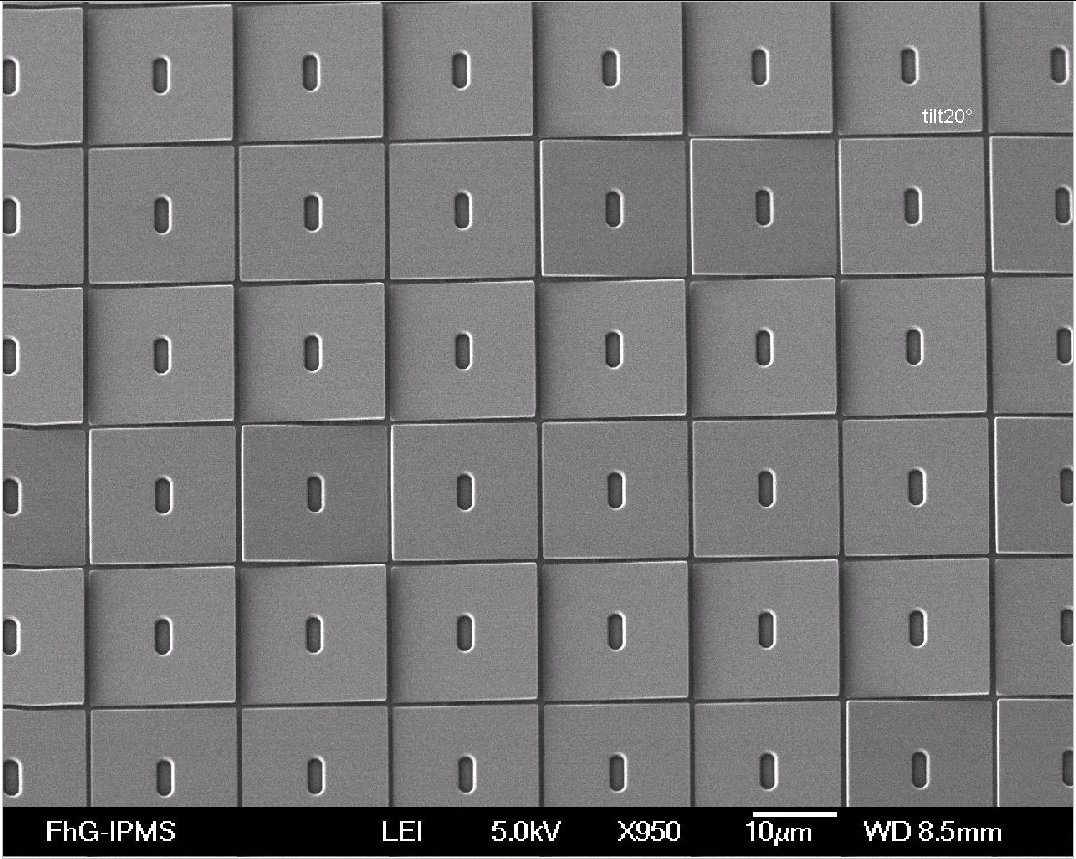
\includegraphics[width=7cm]{mma-tilts}
  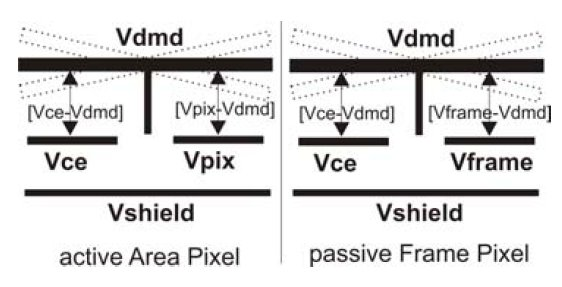
\includegraphics[width=7cm]{mma-voltages}
  \caption{{\bf left:} Electron micrograph showing generation-2 MMA
    with tilted mirrors. {\bf right:} Schematic of the voltages on one
    mirror (both figures by Fraunhofer IPMS).}
  \label{fig:mma-tilts}
\end{figure}
From the beginning of the project a Fourier filtering--based approach
was planned in order to turn the minute tilts of the micro mirrors
into intensity modulations: An aperture is placed on the zero order of
the Fraunhofer diffraction pattern of the MMA. When mirrors are
tilted, they reflect the light outside of the aperture, where it is
absorbed.  This technique has been applied for the generation-0
MMAs. 

However, the Fourier filtering approach has the drawback, that
illumination angles and the size of the aperture are restricted below
the diffraction angles of the MMA. In our optical system this limits
the area on the LCoS, that can be illuminated and therefore the field
of view in the specimen.

A shearing interferometer--based approach was suggested instead. There,
the images of neighbouring mirrors are overlapped and can interfere. A
system based on Wollaston (or Nomarski) prisms would give better
angular acceptance. It promises good contrast and will work for
multiple wavelengths as well.
\section{Description of the setup}
\begin{figure}[ht]
  \centering
  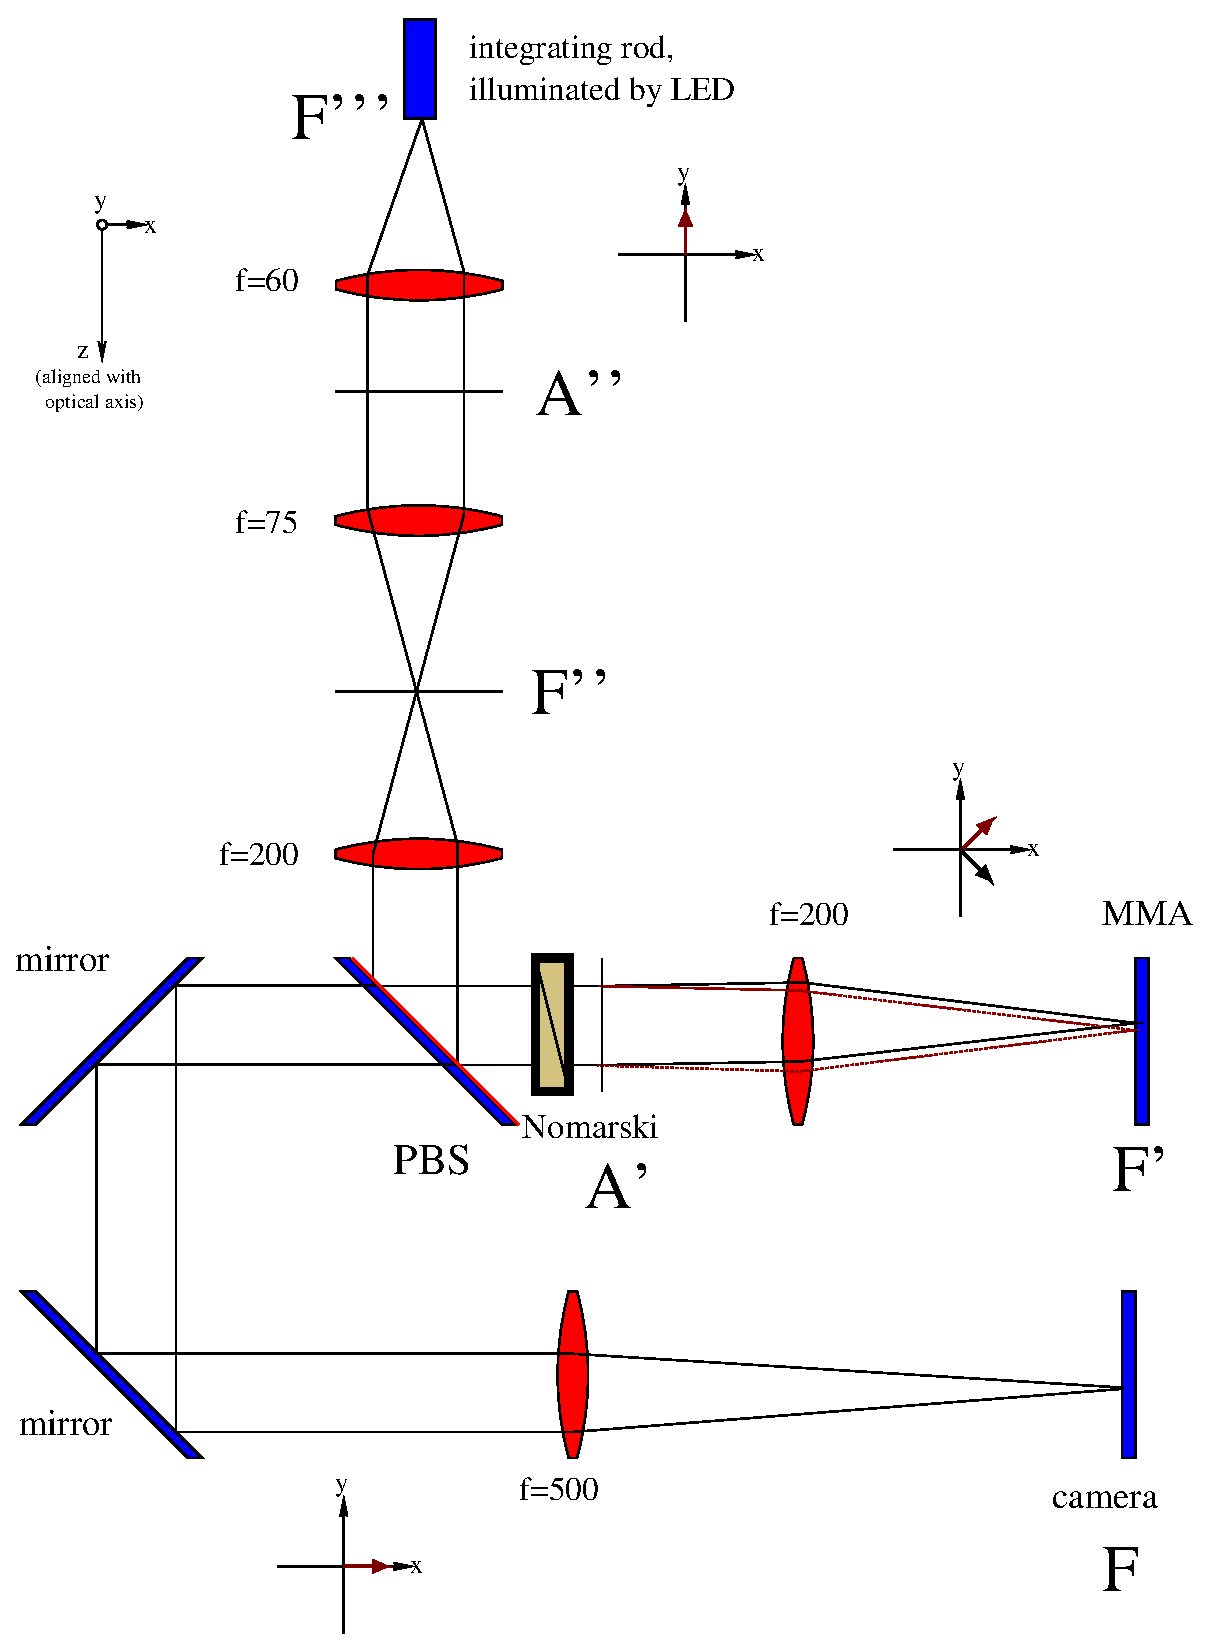
\includegraphics[height=9cm]{../app_dic/img/dic_mma}
  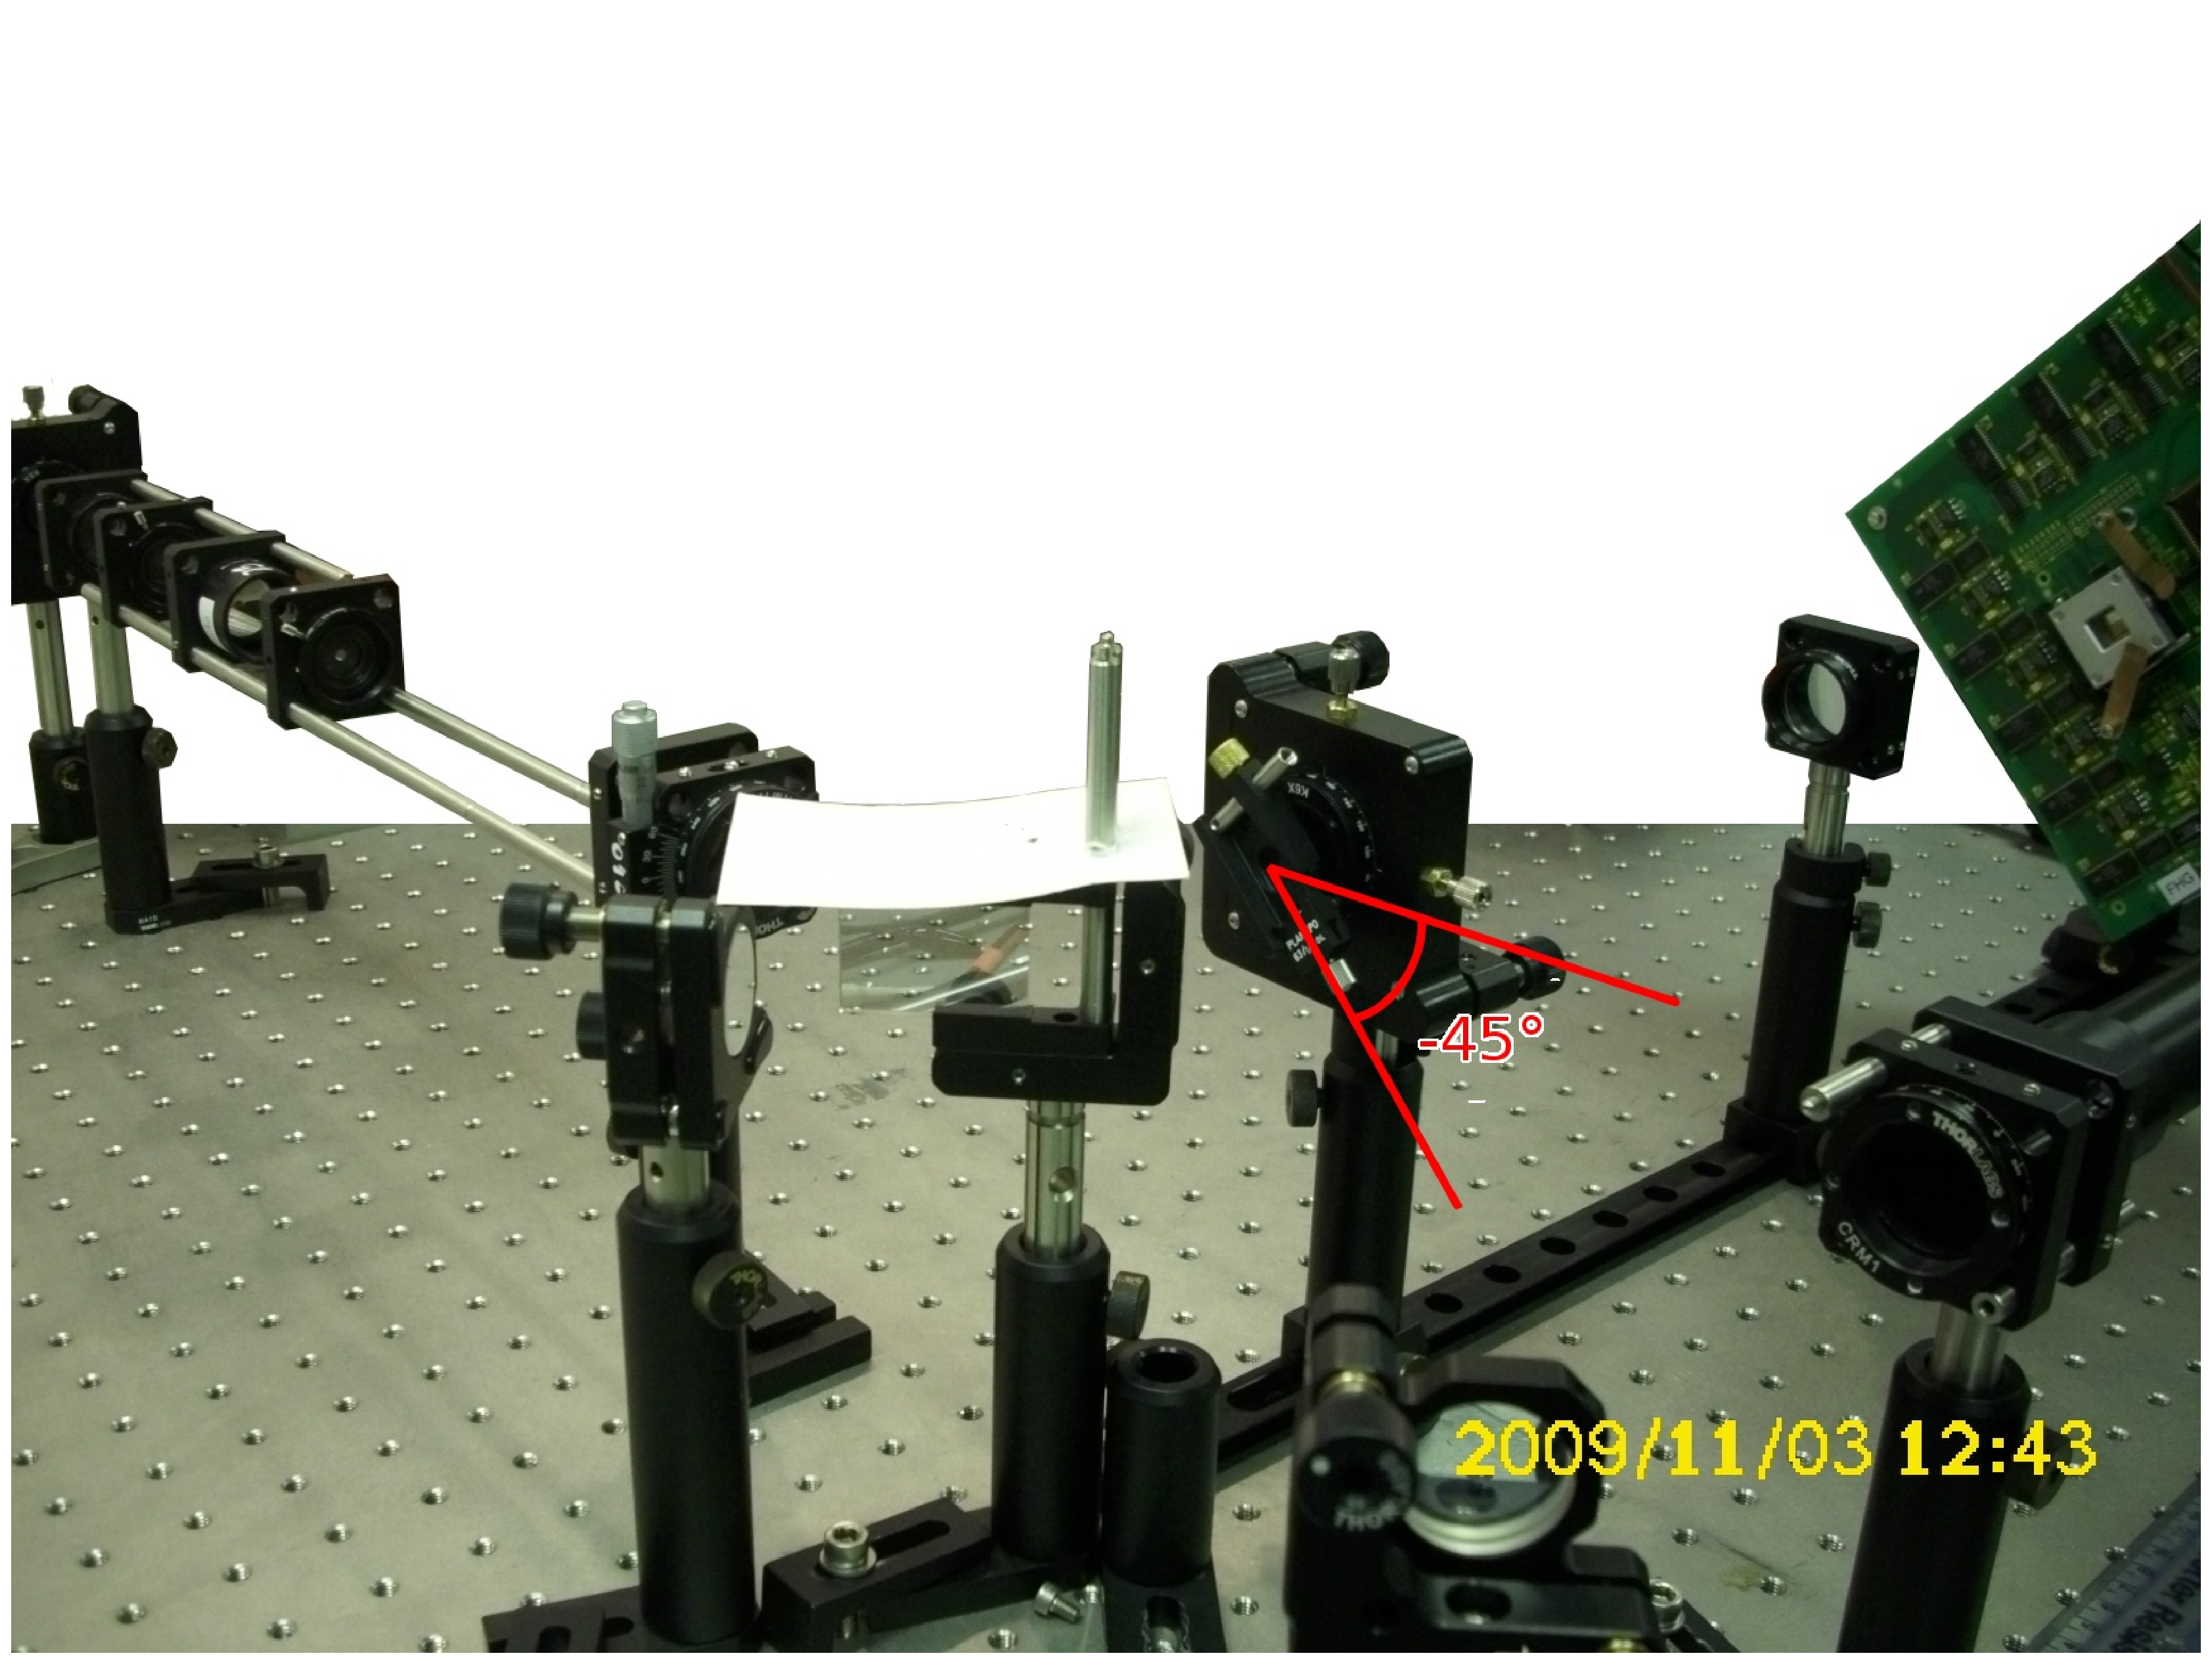
\includegraphics[width=7cm]{../app_dic/img/dsci1331}
  \caption{ Schematic and photograph of the optical setup.  {\bf
      left:} Apertures allow control of the illumination in the planes
    $A''$ and $F''$. The wire grid polarizing beam splitter (PBS) is
    oriented with the aluminium structured side towards the Nomarski
    prism. The Nomarski prism can be rotated around the optical
    axis. Given the orientation of the MMA, the DIC method only works
    for $\pm 45^\circ$ and $\pm 135^\circ$ settings.  {\bf right:}
    Nomarski prism is oriented in $-45^\circ$ direction.  A white
    paper card protects the wire grid polarizer from dust.  This setup
    contains two additional cleanup polarizers that are not shown in
    the schematic in.}
  \label{fig:dic_mma}
\end{figure}
\figref{fig:dic_mma} shows a schematic and a photograph of the setup.
The light source is a liquid light guide--coupled \unit[480]{nm} LED
(CoolLed). It illuminates a square integration rod (\unit[10]{cm}
length) to provide a uniform light distribution in the conjugate
$F'''$ of the field. \nomenclature{DIC}{differential interference contrast}

The optical path for the illumination contains two apertures to
confine the field and to control the illumination angles. We use a
wire grid polarizer (Moxtek, UT, US) as polarizing beam splitter.

Achromatic doublets (objective $f=\unit[200]{mm}$, tubelens
$f=\unit[500]{mm}$) were used as the two imaging lenses.

The position of the focal plane of Nomarski prisms from a Zeiss
microscope was estimated by measuring the distance between the prism
and the back focal plane of the matching micro objectives (the result
is generally within $\unit[2-3]{cm}$). For the fine adjustment of the
prism in our setup, the prism was axially shifted until the dark band
encompasses the full field of view.

We selected the prism with the biggest split angle
($\theta=\unit[0.078]{mrad}$, see section \ref{sec:prism} for the
measurement; matching a $63\times/1.4$ oil immersion objective) in
order to keep the distances small and minimize beam distortion due to
air fluctuations. Later we found that the size of the prism is the
limiting factor. For a good DIC effect at least three orders of the
MMA diffraction pattern have to pass through the prism. To ensure
this, two identical DIC prisms were used sequentially. Note that the
distance between the prisms allows to vary the split angle
\citep{Schwertner2008}.

The objective lens and the MMA are positioned on a rail to simplify
focusing. The lens positions were pairwise adjusted by sending a
plane wave of a green laser through each ``telescope'' and moving one
lens until the outgoing wave was plane (using a shear plate). The
distance of tube lens and camera was set to the focal length by
reflecting a parallel beam into the tube lens and minimizing the size
of the spot on the camera.

\section{Displaying arbitrary gray values using the DIC approach}
\begin{figure}[htb]
  \centering
  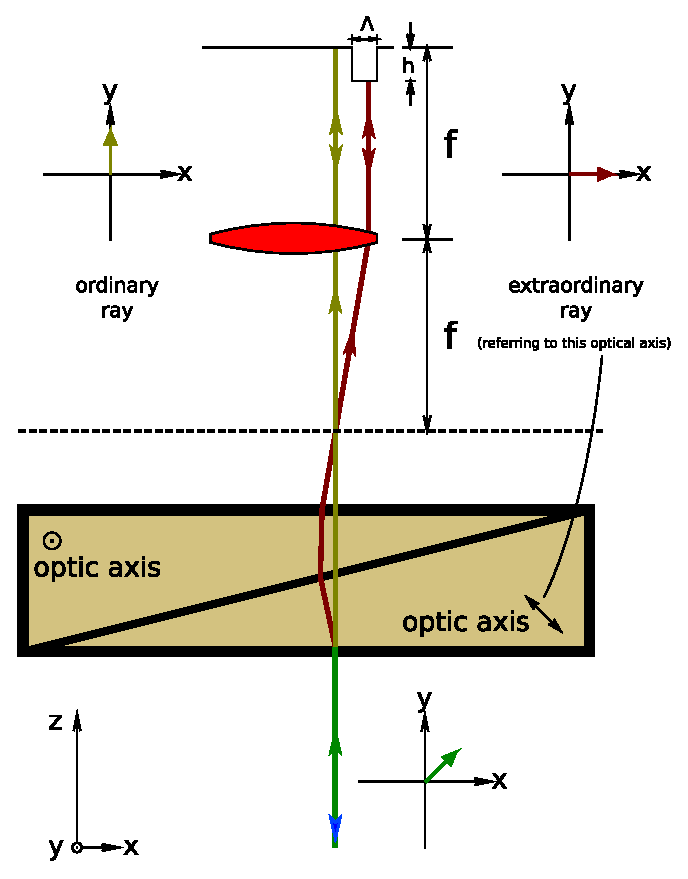
\includegraphics[width=6cm]{../app_dic/img/dic_prism}
  \caption{ Linearly polarized light is split by the prism into two
    rays with slightly diverging angle. They hit the MMA at two spots,
    which are one shearing distance apart. The light returning through
    the Nomarski prism has different polarization states depending on
    the height difference $h$ of the mirrors at those two beam
    positions.}
  \label{fig:prism}
%http://www.microscopy.fsu.edu/primer/java/polarizedlight/crystalwavefronts/index.html
\end{figure}
First we consider a simplified arrangement of one piston micro mirror
of width $\Lambda$ on a plane mirror (see \figref{fig:prism}).  Let
$k=2\pi/\lambda_0$ with vacuum wavelength $\lambda_0$. We write the
influence of a retarder (the height difference $h$ of the small piston
mirror) on a polarized wave in Jones calculus as (\cite{Goodman1996}
p.~418):
\begin{align}
L_r(\Delta)=\begin{pmatrix}1&0\\ 0&e^{-i\Delta}\end{pmatrix}
\end{align}
with a phase difference $\Delta=2kh$ (the factor 2 due to the
reflection).  The matrix for a polarizer that passes the component of
the electrical field which is linearly polarized at an angle $\alpha$
to the x-axis is:
\begin{align}
L_p(\alpha)=\begin{pmatrix}\cos^2\alpha&\sin\alpha\cos\alpha\cr
  \sin\alpha\cos\alpha&\sin^2\alpha\end{pmatrix}.
\end{align}
In our setup the incoming light has a $45^\circ$ polarization $\vect
U=(1,1)^T/\sqrt{2}$ after the first reflection on the PBS. The light
passes through the Nomarski prism and is reflected by the MMA. Here
depending on the mirror height a phase retardation is imposed on one
of the two beams. The reflected light is recombined in the Nomarski
prism and only the component that is polarized at $\alpha=-45^\circ$
passes through the PBS onto the camera: $\vect
U'=L_p(-45^\circ)L_r(\Delta)$.
\begin{align}
  I'=|\vect U'|^2=(1-\cos\Delta)/2
\end{align}
The camera image is dark for a plane mirror and is maximal for a
piston height $h=lambda/4$.
%a:-%pi/4;
%r:matrix([1,0],[0,exp(-%i*d)]);
%p:matrix([cos(a)^2,sin(a)*cos(a)],[sin(a)*cos(a),sin(a)^2]);
%expand((p . r . [1,1]) . conjugate(p . r . [1,1]));
For a piston mirror of width $\Lambda$ the intensity of the
corresponding pixel on the camera is (assuming it receives all the
light from one mirror):
\begin{align}
  I_p=\int_{-\Lambda/2}^{\Lambda/2} I'(\Delta(x'))\textrm{d}x'=\frac{\Lambda}{2}(1-\cos \Delta).
\end{align}
\begin{figure}[ht]
  \centering
  \includegraphics[width=7cm]{../app_dic/img/tilt}
  \caption{ Two mirrors that tilt with different deflections $d_1$ and
    $d_2$ in opposite directions. The pitch of the mirrors is
    $\Lambda$.}
  \label{fig:tilt}
\end{figure}
As the mirrors of the MMA tilt (and don't move like pistons) it is
necessary to integrate along the DIC shift direction $x'$ to get the
brightness of one pixel depending on the tilt of the two neighbouring
mirrors (this calculation is done for small mirror tilts, see
\figref{fig:tilt}): 
% Delta = 2kh; 
% integrate((1-cos(2kh))/2,x,-l/2,l/2);
% h(l) = d, h(-l) = d, h(0) = 0
% h(x) = abs(d*x/l) 
% 2*integrate((1-cos(2*k*d*x/l))/2,x,0,l/2);
\begin{align}
\label{eqn:it}
  I_t=\int_{-\Lambda/2}^{\Lambda/2} I'(\Delta(x')) \textrm{d}x'=\frac{\Lambda}{2}\left(1-\frac{\sin(k \Delta d)}{k \Delta d}\right).
\end{align}
Here $\Delta d=d_1-d_2$ is the difference between the deflections
$d_1$ and $d_2$ of the two mirrors and $\Lambda$ is the mirror pitch
(see \figref{fig:tilt}). Note that the integral sums incoherently
across the mirror because in our experiment we use a LED light
source. Note that the DIC image of torsion mirrors is in general not
constant over the width $\Lambda$ of one mirror. Neighbouring mirrors
do not differ in their height at the positions where they are
fixed. Therefore there will always be a dark stripe in the centre of
the mirrors. This artifact wouldn't occur with piston style mirrors.

The scale factor of $I_t$ is arbitrary. In order to get a more useful
result we compare the brightness of MMA mirrors $I_t$ to a theoretical
device consisting of pistons that can move the distance $d$ away from
the equilibrium position:
\begin{align}
\label{eqn:eta}
  \eta(\Delta d)=\frac{I_t}{I_p}=\frac{1-\sin(k\Delta d)/(k\Delta d)}{1-\cos(2kd)}.
\end{align}
\begin{figure}[ht]
  \centering
  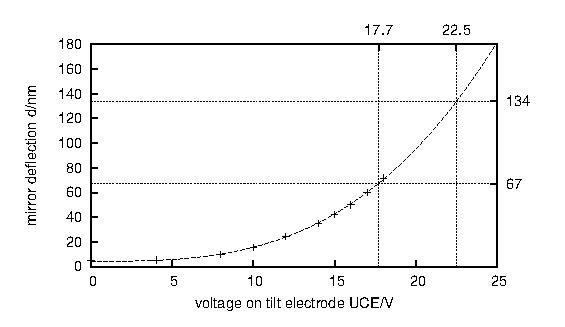
\includegraphics{../app_dic/img/plot/deflection}
  \caption{Deflection curve for our generation-0 MMA sample (data
    supplied by Fraunhofer IPMS) and corresponding fit of cubic
    polynomial $d=a\cdot x^3+b$ with $a=\unit[(0.01136\pm0.0001)]{nm\,
      V^{-3}}$ and $b=\unit[(4.32\pm0.3)]{nm}$. The x-axis is the
    voltage $U_\textrm{CE}$ that is applied to one of the electrodes
    of the mirror and the y-axis shows the deflection $d$ of the
    mirror (distance from mirror edge to the equilibrium
    position). The maximum voltage that we apply to the mirrors in our
    experiments is \unit[22.5]{V}.}
  \label{fig:deflection}
\end{figure}
The data sent to the generation-0 MMA are integers $q\in[0,255]$
that set the voltage of the counter electrode $U_\textrm{CE}$
\begin{align}
U_\textrm{CE}(q)=s_\textrm{img}\cdot \unit[30]{V} \cdot \frac{q}{255}.
\end{align}
The scale factor $s_\textrm{img}$ is \unit[0.75]{} in our experiments.
Fraunhofer provides a transfer function for the MMA that describes the
relation between the voltage and the deflection (see
\figref{fig:deflection}) from 0 to $U_\textrm{CE}=\unit[18]{V}$. They
also request, not to use any voltages higher than \unit[22.5]{V}. If
the extrapolation to higher deflections is correct, then the maximum
deflection is: % k:2*%pi/480; plot2d((1-sin(k*x)/(k*x))/(1-cos(2*k*134)),[x,0,134]);
\begin{align}
\label{eqn:dmax}
d_\textrm{max}=\unit[0.01136]{\frac{nm}{V^3}}\cdot(0.75\cdot\unit[30]{V})^3+\unit[4.32]{nm}
=\unit[(134\pm2)]{nm}.
\end{align}
For a wavelength of \unit[480]{nm} the maximum $\eta$ we can achieve
is $0.21$. Therefore for this wavelength and this particular
generation-0 MMA, pistons instead of torsion mirrors would achieve
five times higher contrast (assuming the piston can only move in one
direction from the plane of equilibrium).
\begin{figure}[ht]
  \centering
  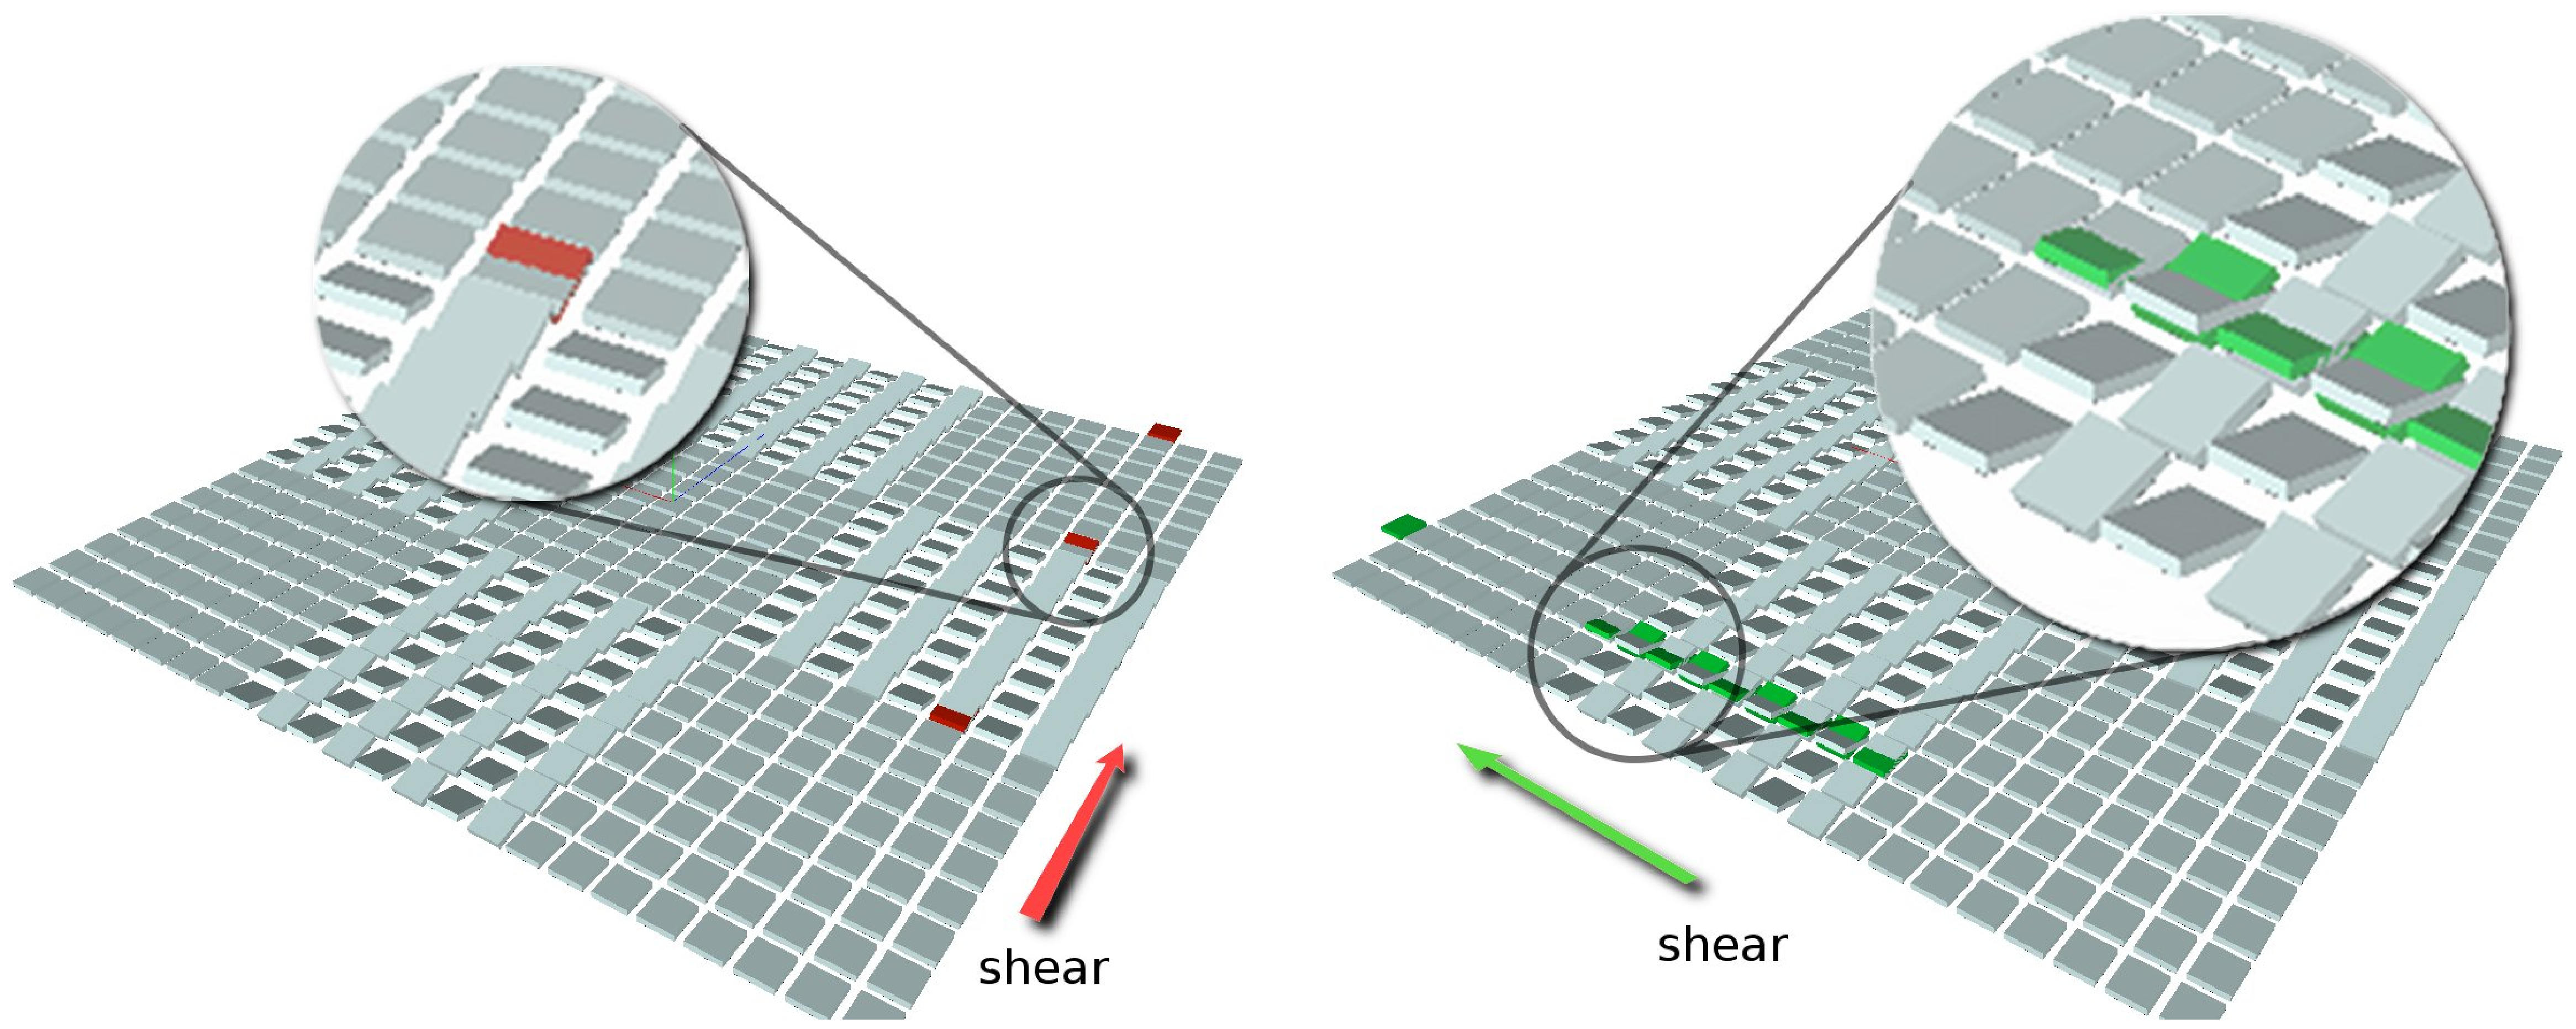
\includegraphics[width=\linewidth]{../app_dic/img/mma_sketch}
  \caption{ Diagrams showing how rows (Nomarski prism in $-45^\circ$
    angle, left) or columns (Nomarski prism in $+45^\circ$, right) of
    the MMA are overlaid by the DIC prism. The coloured parts depict
    the neighbouring mirror as it is overlaid by the DIC. These
    images only show a $24\times 24$ section of mirrors with a
    checkerboard of $16\times 16$ periodicity.}
  \label{fig:screen}
\end{figure}
\begin{figure}[htb]
  \centering
  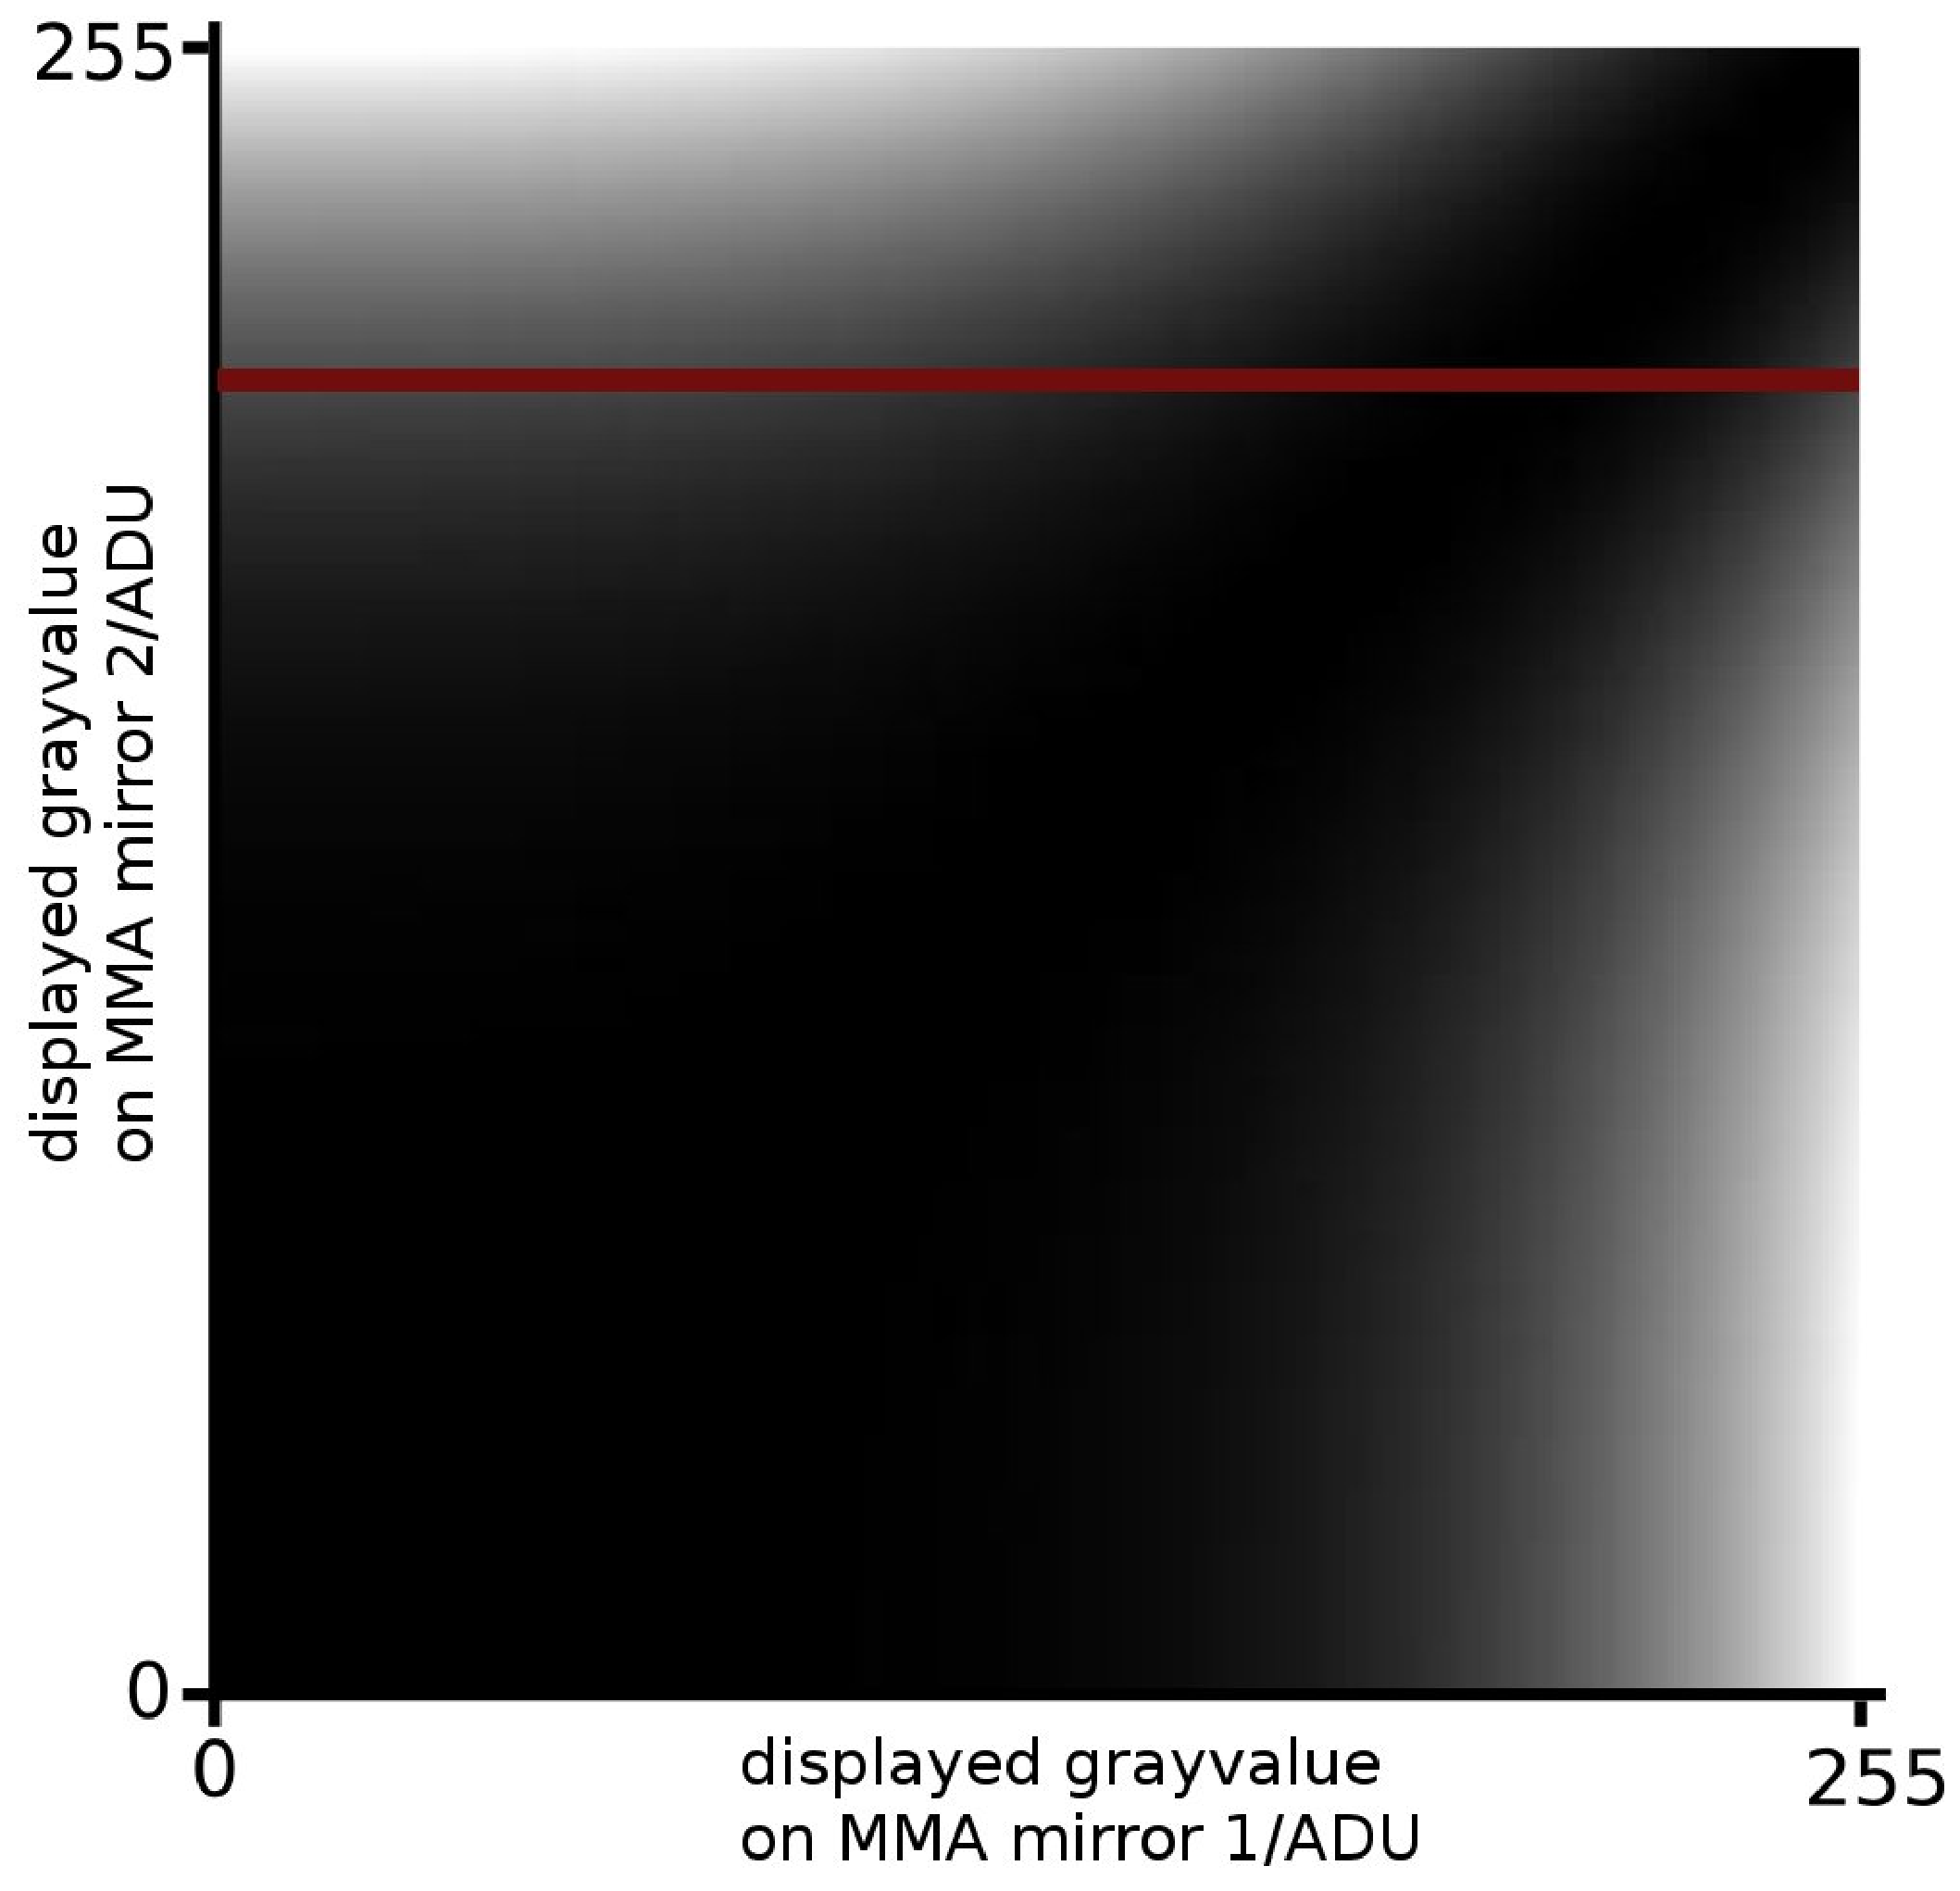
\includegraphics[height=6.5cm]{../app_dic/img/lut-plot}
  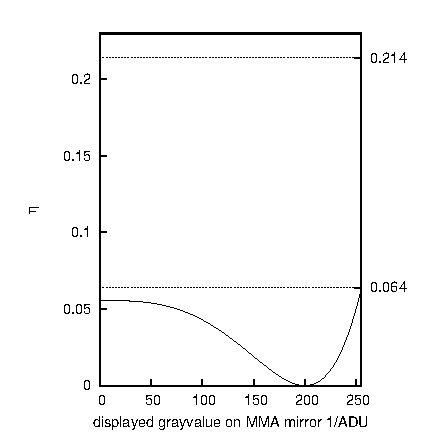
\includegraphics[height=6.5cm]{../app_dic/img/plot_lut/lut_graph}
  \caption{{\bf left:} Theoretical $\eta$ in dependence of the tilts
    of neighbouring mirrors. The analog-digital units (ADU) are
    proportional to the voltage $U_\textrm{CE}$. An ADU of 255
    corresponds to a deflection of \unit[134]{nm}. Black corresponds
    to $\eta=0$ and white corresponds to $\eta=0.21$. {\bf right:} The
    graph shows the values along the red line in the matrix on the
    left, i.e. ``mirror 2'' is not tilted with gray value~200
    corresponding to a tilt voltage $U_\textrm{CE}=\unit[17.7]{V}$
    that deflects the mirror to half of the maximum possible
    deflection. The maximum brightness $\eta=0.064$ that can be
    obtained with this setting (when ``mirror 1'' is tilted to the
    maximum angle) is $30\%$ of the brightness for maximum tilt
    difference between two mirrors.}
  \label{fig:deflection2}
\end{figure}

Due to the bidirectional tilt of the mirrors along alternating rows
(see \figref{fig:screen}) the MMA allows two different DIC modes.
Either the mirrors are overlaid along rows (all mirrors tilt into the
same direction, see the left image in \figref{fig:screen}) or mirrors
are overlaid in column direction (neighbouring mirrors tilt to
opposite sides, see the right image in \figref{fig:screen}). The
latter mode we cannot employ to display arbitrary images.  Two
neighbouring flat mirrors will produce black and two opposite-tilt
mirrors will produce a maximum. There is no way how these mirror tilts
can be adjusted such, that arbitrary gray value images can be
generated -- which is our goal.

However, when the DIC shear direction is the same as the mirror tilt direction
it is indeed possible to display arbitrary gray value images.

We generate a black image pixel by setting two immediate neighbours to
the same tilt angle. We create arbitrary gray values by tilting
neighbouring mirrors in slightly different directions. Equation
\eqref{eqn:it} describes the relation between tilts of the mirrors and
the intensity of the image pixel. The brightest value
$\eta=0.214$\todo{wrong}\ can be achieved when one mirror is flat and
the neighbour is tilted to the maximum possible deflection
$d_\textrm{max}$ (equation \eqref{eqn:dmax} shows its value for our
generation-0 MMA).  However, it is not possible to exploit the full
dynamic range of the device when arbitrary images are to be displayed
(at least not with the algorithm that we are going to describe).
Instead the maximum dynamic range is from $\eta=0$ to $\eta=0.064$.

The algorithm that we use to calculate the mirror tilts -- or rather
the pixel values $q$ -- that will result in a given intensity image
after the DIC device. It uses our model of the DIC device and the
transfer function that maps voltages to mirror tilts.

Set a pixel on the border of the MMA to 0. We call this pixel ``mirror
2''. Then go one pixel in the direction of the DIC shift. We call this
pixel ``mirror 1''. Look in the target image what intensity should be
produced at this position. Search this intensity in the look up table
(\figref{fig:deflection2}) along the abscissa (for gray value 0 of
``mirror 2'') and set the gray value of ``mirror 1'' to the
corresponding gray value. Now rename ``mirror 1'' to ``mirror 2'' and
go to the next pixel of the matrix. Repeat this procedure for all
pixels in this rows and do this algorithm for all columns of the MMA.

When the shear induced by the Nomarski prism doesn't equal the mirror
pitch of \unit[16]{$\mu$m}, then the interference image of two
mirrors will be deteriorated by line like artifacts on the sides.

\section{Experimental results}
\subsection{Procedure to measure the split angle of a Nomarski prism}
\label{sec:prism}
The Nomarski prism consists of two quartz wedges. Its function is
based on the birefringence of the crystal. The prism splits a
$45^\circ$ linearly polarized wavefront into two wavefronts with
slightly diverging angles.
\begin{figure}[htb]
  \centering
  \includegraphics[width=8cm]{../app_dic/img/nomarski_split}
  \caption{Setup to measure the split angle $\theta$ of a Nomarski
    prism by interference of the two beams. The polarizers Pol1 and
    Pol2 are crossed and in a $45^\circ$ angle relative to the shift
    axis of the prism.}
  \label{fig:nomarski_split}
\end{figure}
The split is so small that its direct measurement --- illuminating the
prism with a parallel beam and putting the camera into the back focal
plane of a lens with a long focal length --- is difficult.  Instead we
put the prism between crossed polarizers, illuminate it with a
parallel beam and measure a fringe pattern on the camera (see
\figref{fig:nomarski_split} for a schematic of the setup and
\figref{fig:nomarski_split_exp} for the data).

The electrical field $U$ after the second polarizer is:
\begin{align}
  U&=e^{i\vect k_1\vect r}+e^{i\vect k_2\vect r},\\
  \abs{\vect k}&=\frac{2\pi}{\lambda},\\
  \vect k_1&=\abs{\vect k}(0, \hspace{1em}\sin(\theta/2), \cos(\theta/2))^T,\\
  \vect k_2&=\abs{\vect k}(0, -\sin(\theta/2), \cos(\theta/2))^T.
\end{align}
The camera measures the intensity $I$:
\begin{align}
  I=\abs{U}^2=4\cos^2(\abs{\vect k}y\sin(\theta/2)).
\end{align}
Therefore the dark bands have a distance $d$ (for small split angles
$\theta$):
\begin{align}
  d=\frac{\lambda}{2\sin{\theta/2}}\approx \frac{\lambda}{\theta}.
\end{align}
\begin{figure}[htb]
  \centering
  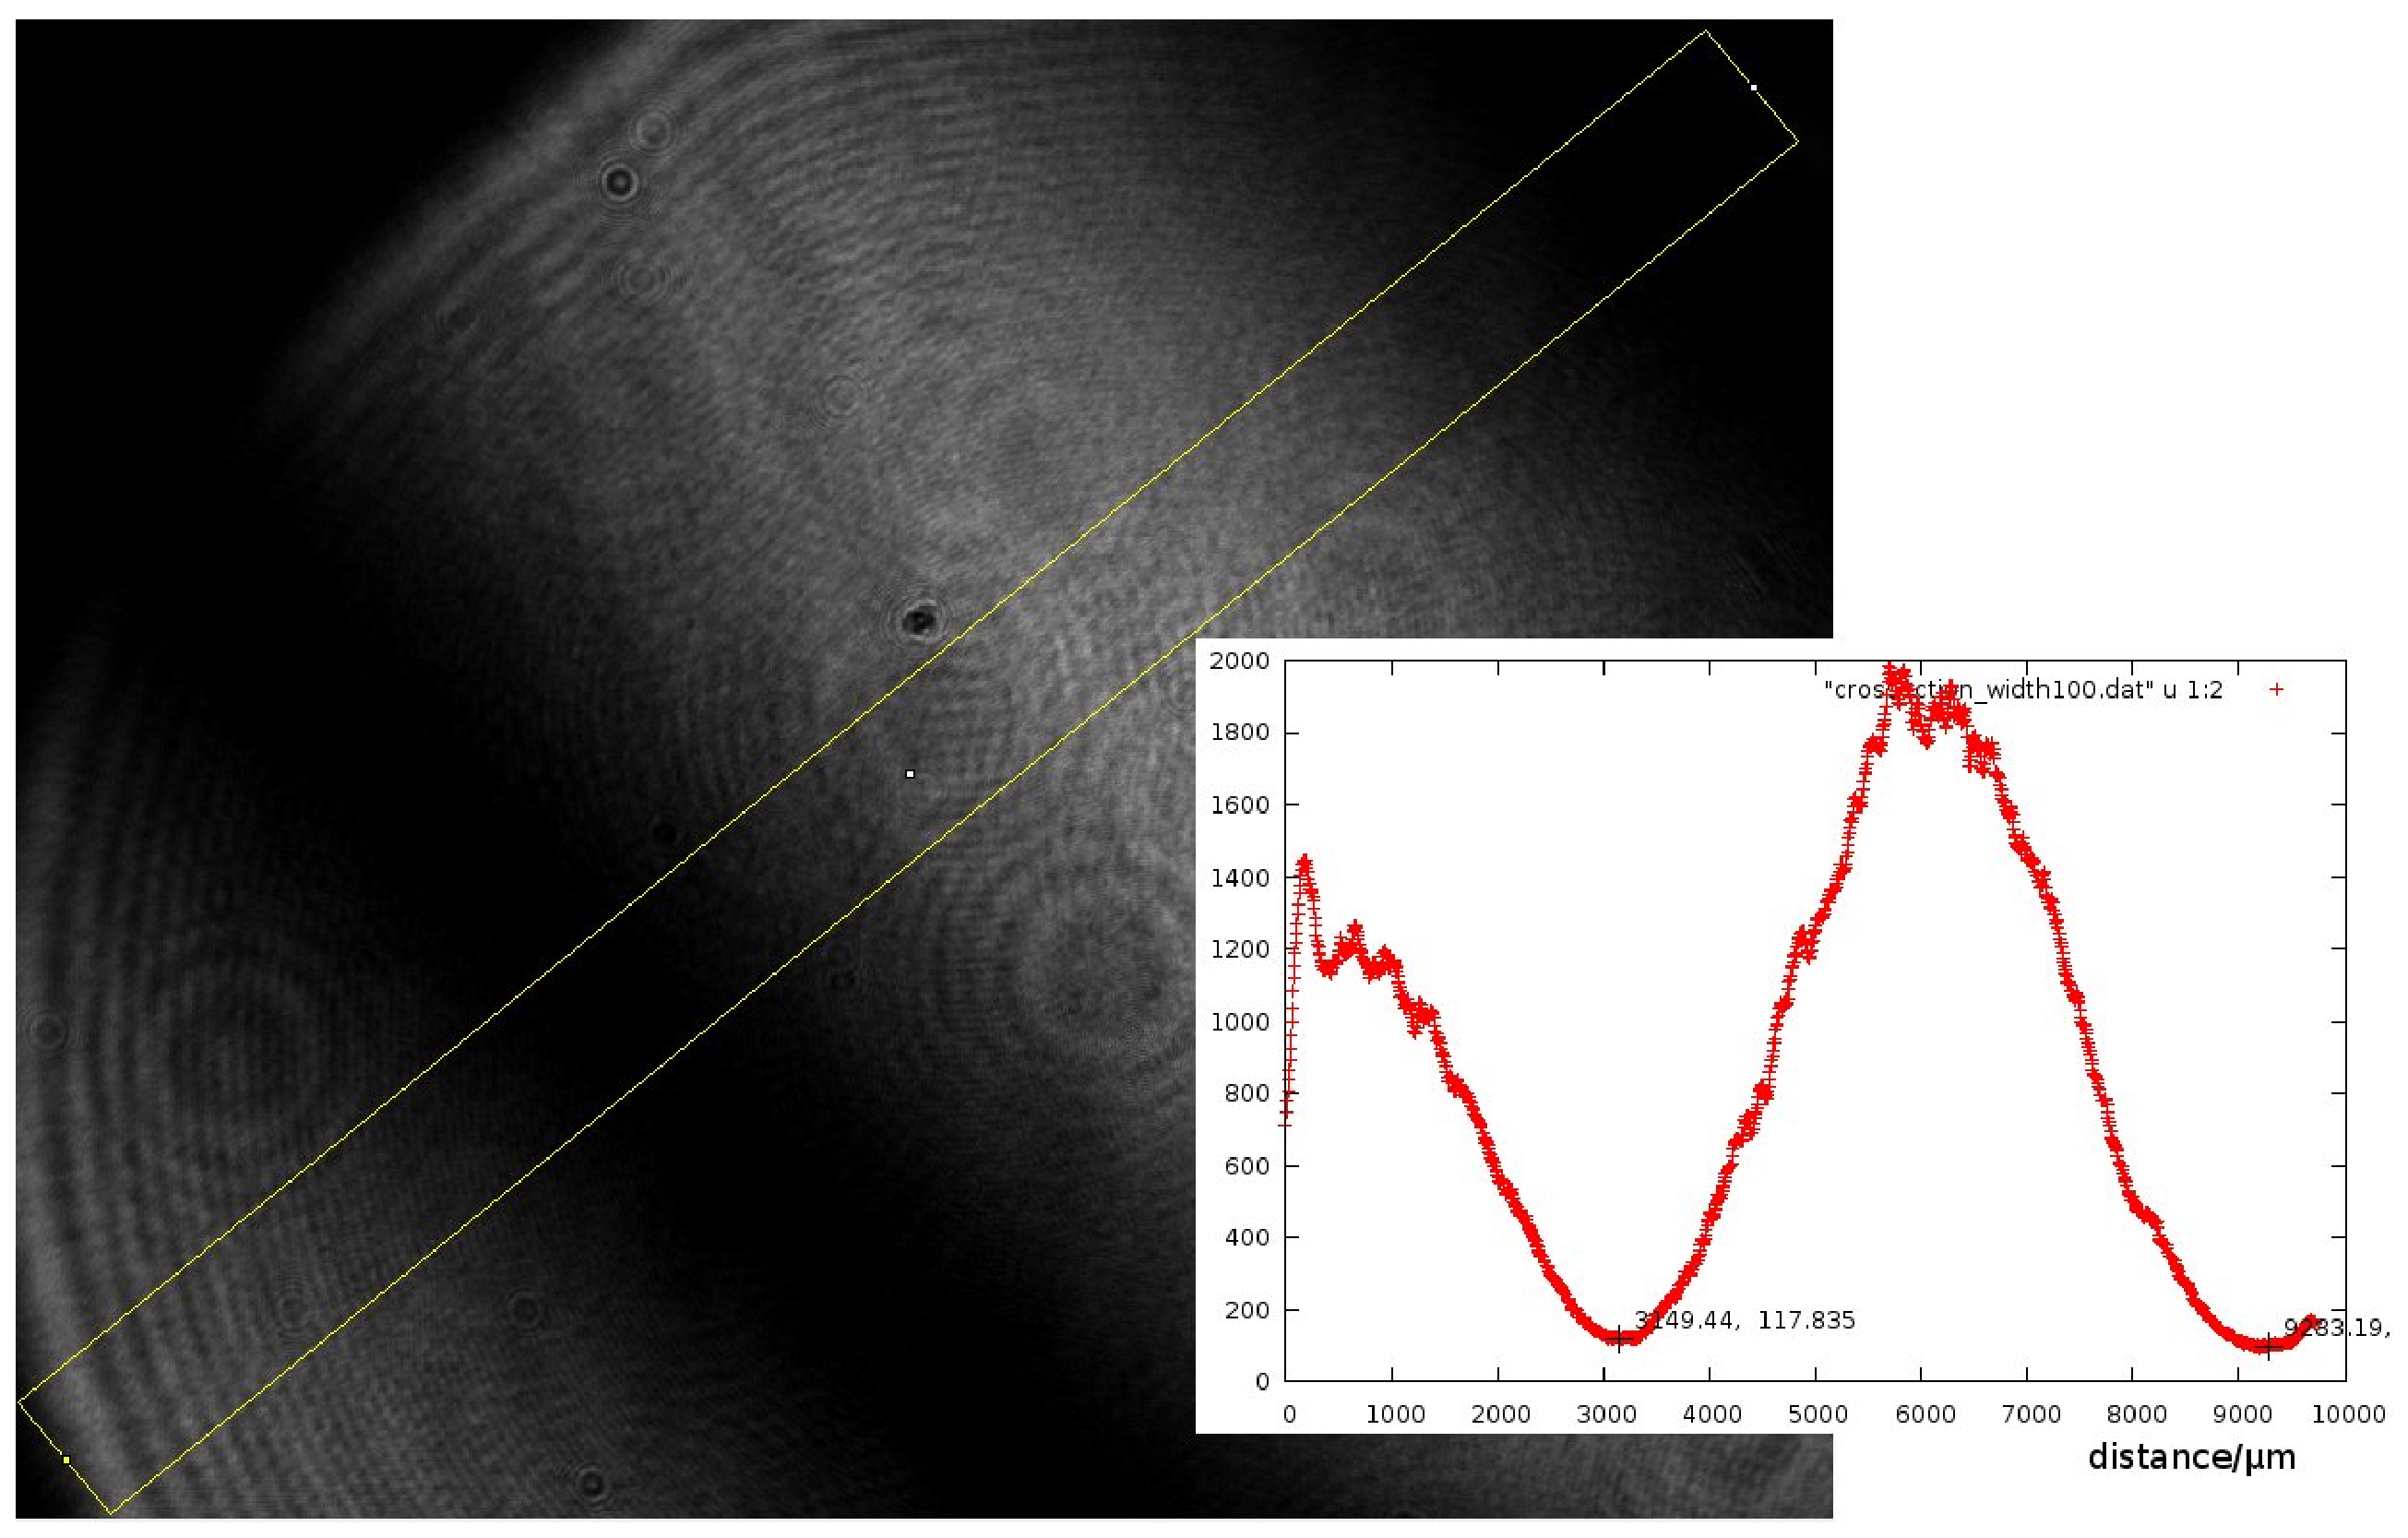
\includegraphics[width=10cm]{../app_dic/img/nomarski_split_exp}
  \caption{Camera image for the prism with the biggest split. The
    distance between the two dark fringes is
    $d=\unit[(6.06\pm0.08)]{mm}$. The light source is a laser with
    \unit[473]{nm} wavelength. The values were integrated over the
    width of the yellow bar to reduce the influence of the disturbing
    fringes on the cross section.}
  \label{fig:nomarski_split_exp}
\end{figure}
Our prism has a split angle $\theta=\unit[0.078]{mrad}$.
For a lens with a focal distance $f=\unit[200]{mm}$ this corresponds to a
Nomarski split $\Delta x$:
\begin{align}
  \Delta x=2f\tan(\theta/2)\approx f\theta=\unit[(15.6\pm0.2)]{\mu m}.
\end{align}
This is close to the pixel pitch of $\unit[16]{\mu m}$ of the MMA.

\subsection{Imaging the MMA with the DIC method}
\figref{fig:screen5} shows see two typical images that can be
achieved with the DIC setup. On these images the mirrors of the MMA
tilt in $-45^\circ$ (to the bottom right) or in $+135^\circ$ (to the
top left).

The image that is displayed on the MMA for both pictures is a black
and white checkerboard with a periodicity of $16\times16$ elements (as
in \figref{fig:screen}).  \figref{fig:screen5}~b) contains the case
that is not usable for us. The DIC shift is along the $+45^\circ$
direction and brings mirrors that tilt in different directions to
interference.  The parts of the checkerboard pattern, where the
mirrors are tilted appear bright in this image. The regions where the
mirrors are flat are dark in the image. According to the right diagram
in \figref{fig:screen} the bright rectangles should have a darker
border. Indeed this can be seen in the image on the camera (indicated
by purple arrow in bottom right of \figref{fig:screen5}).

\begin{figure}[p]
  \centering
  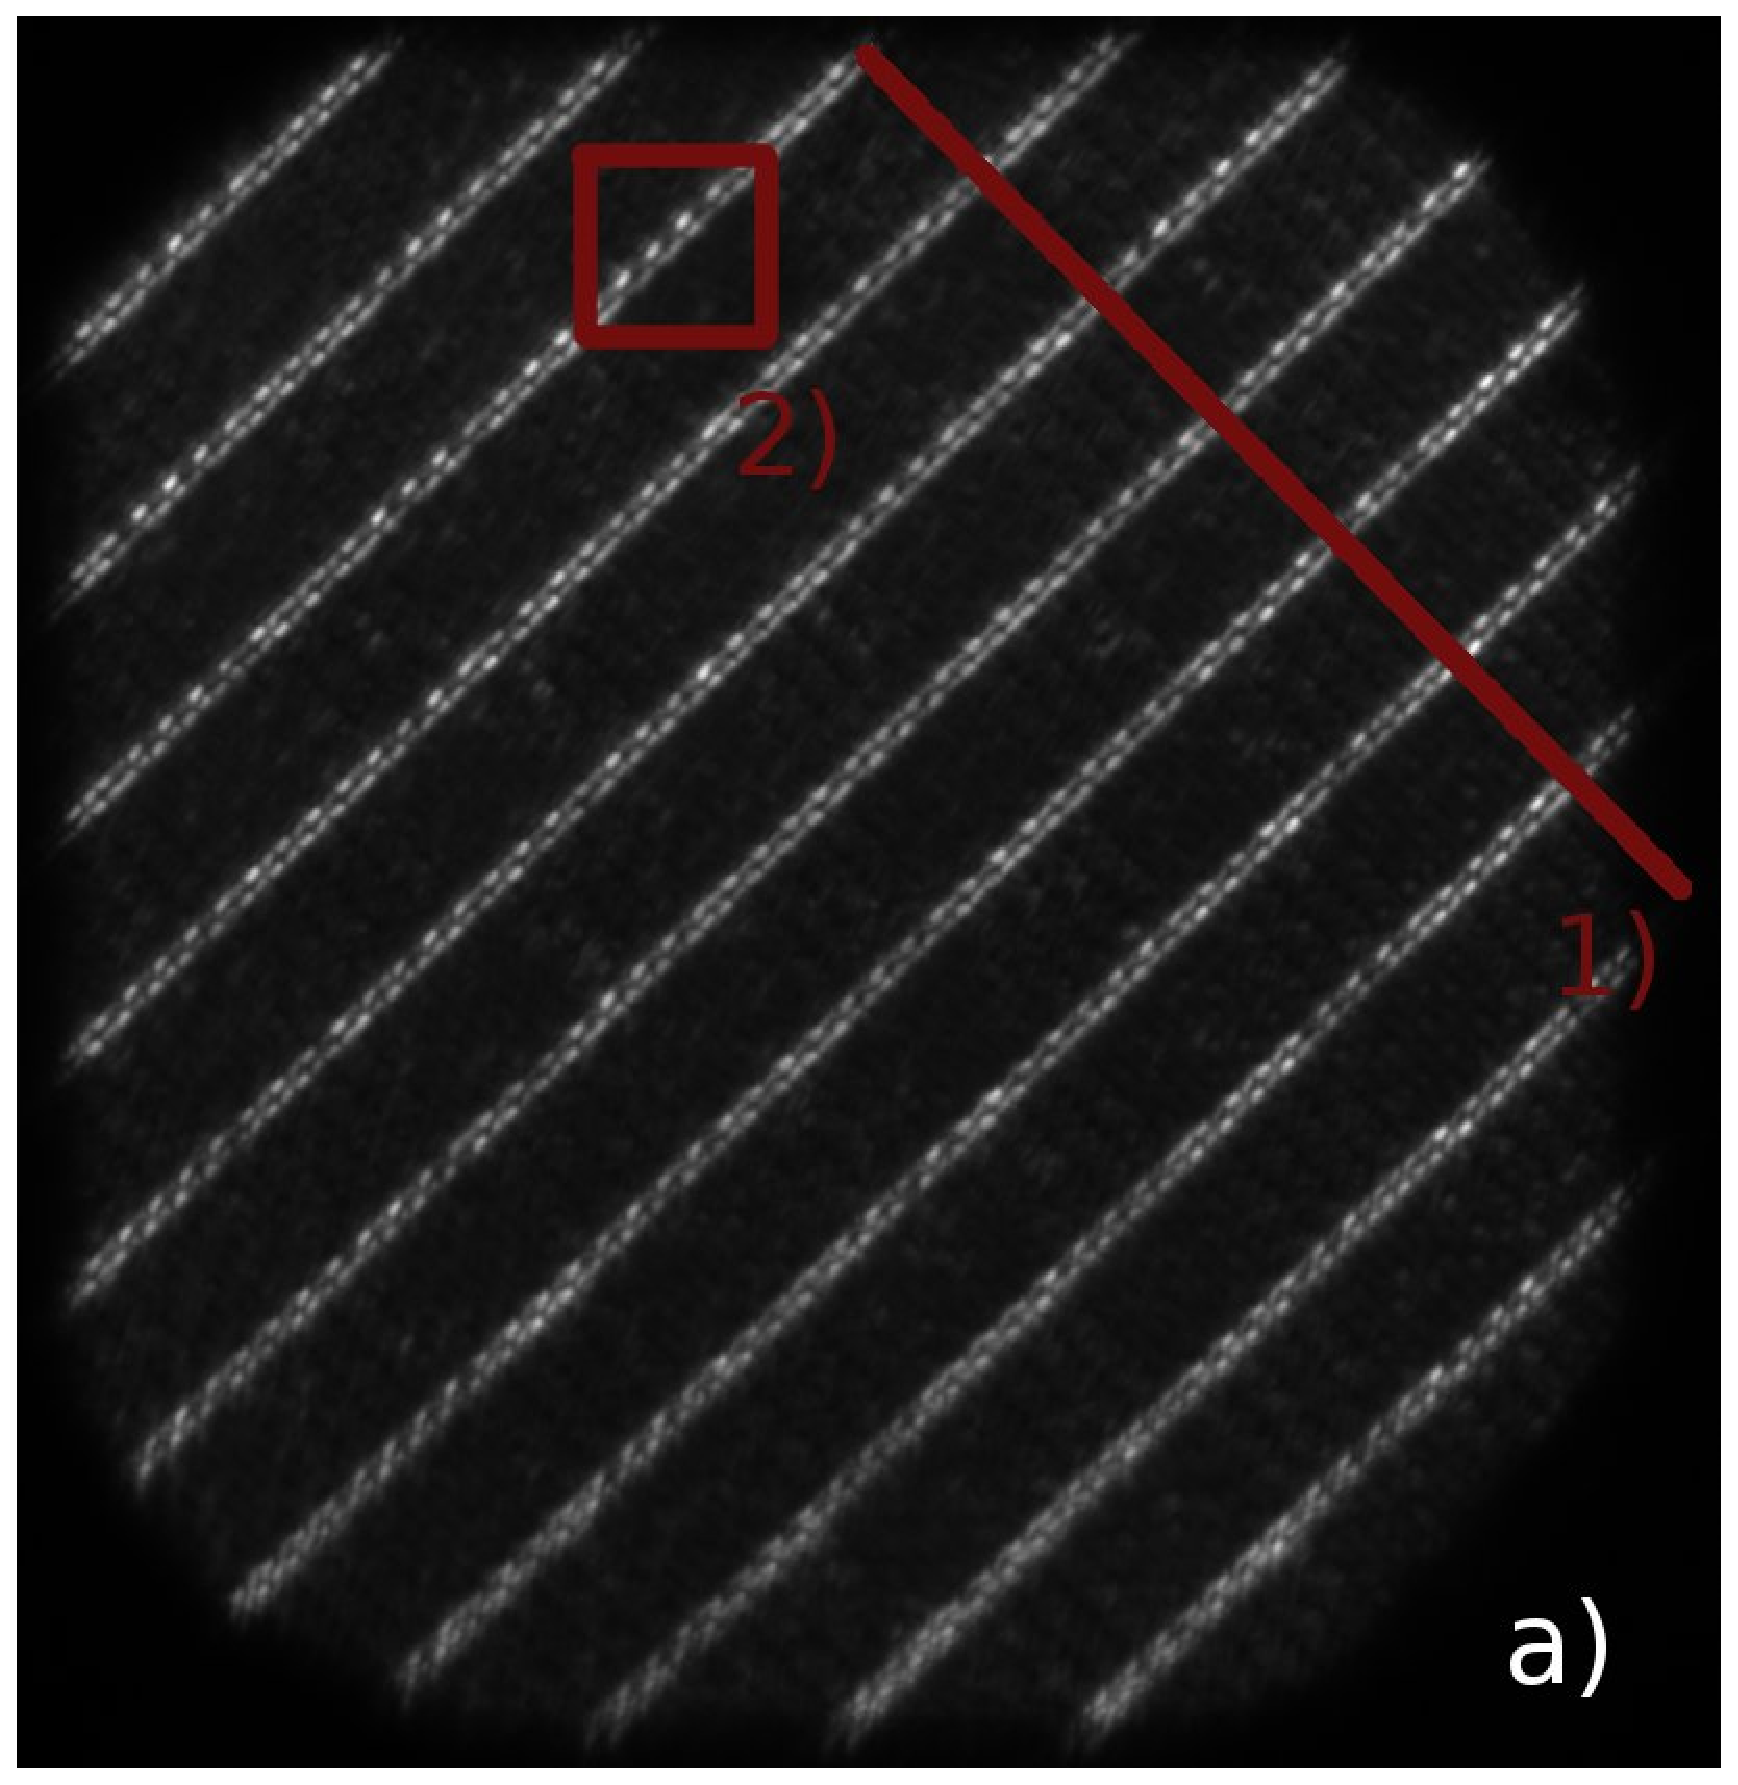
\includegraphics[height=5.9cm]{../app_dic/img/1219/auswert/1checker}
  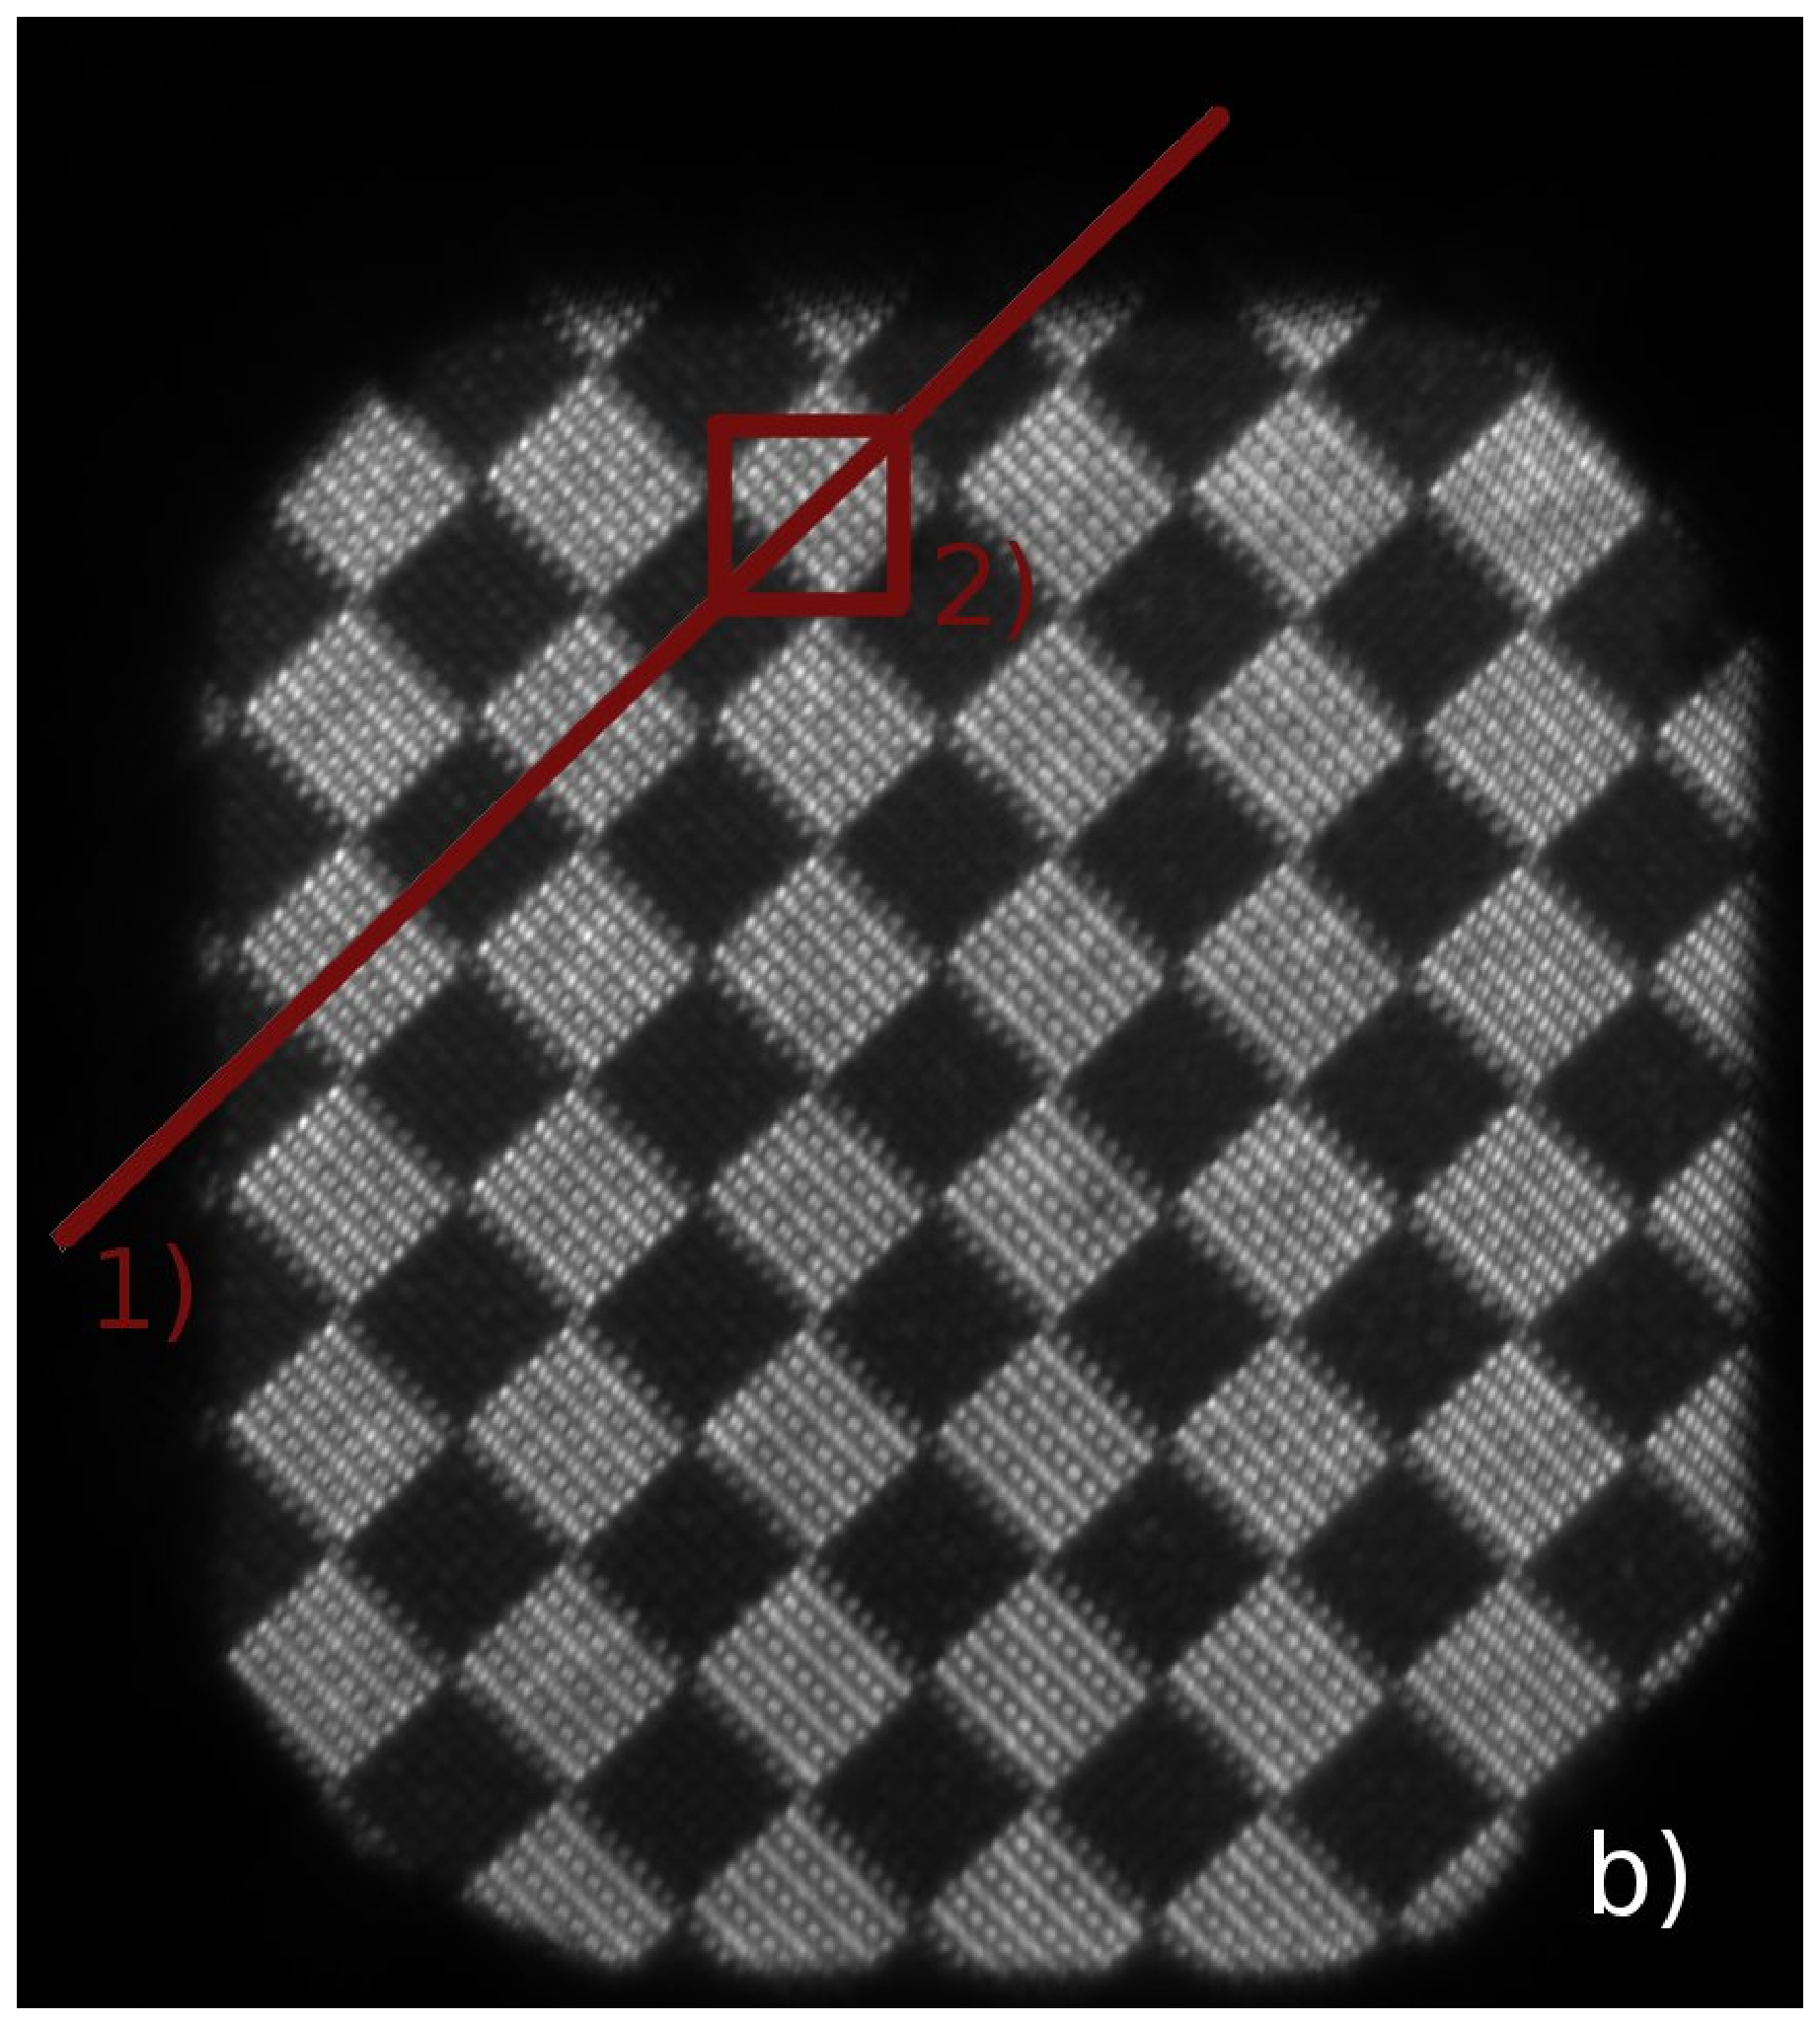
\includegraphics[height=5.9cm]{../app_dic/img/1219/auswert/2checker}
  
\includegraphics[width=7cm]{../app_dic/img/1219/auswert/1checker-section}
  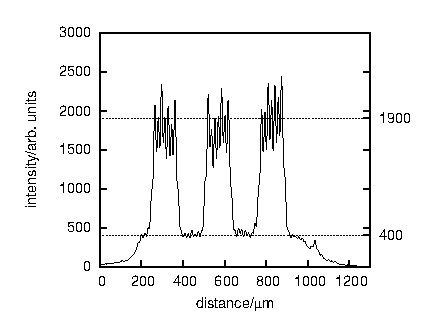
\includegraphics[width=7cm]{../app_dic/img/1219/auswert/2checker-section}
  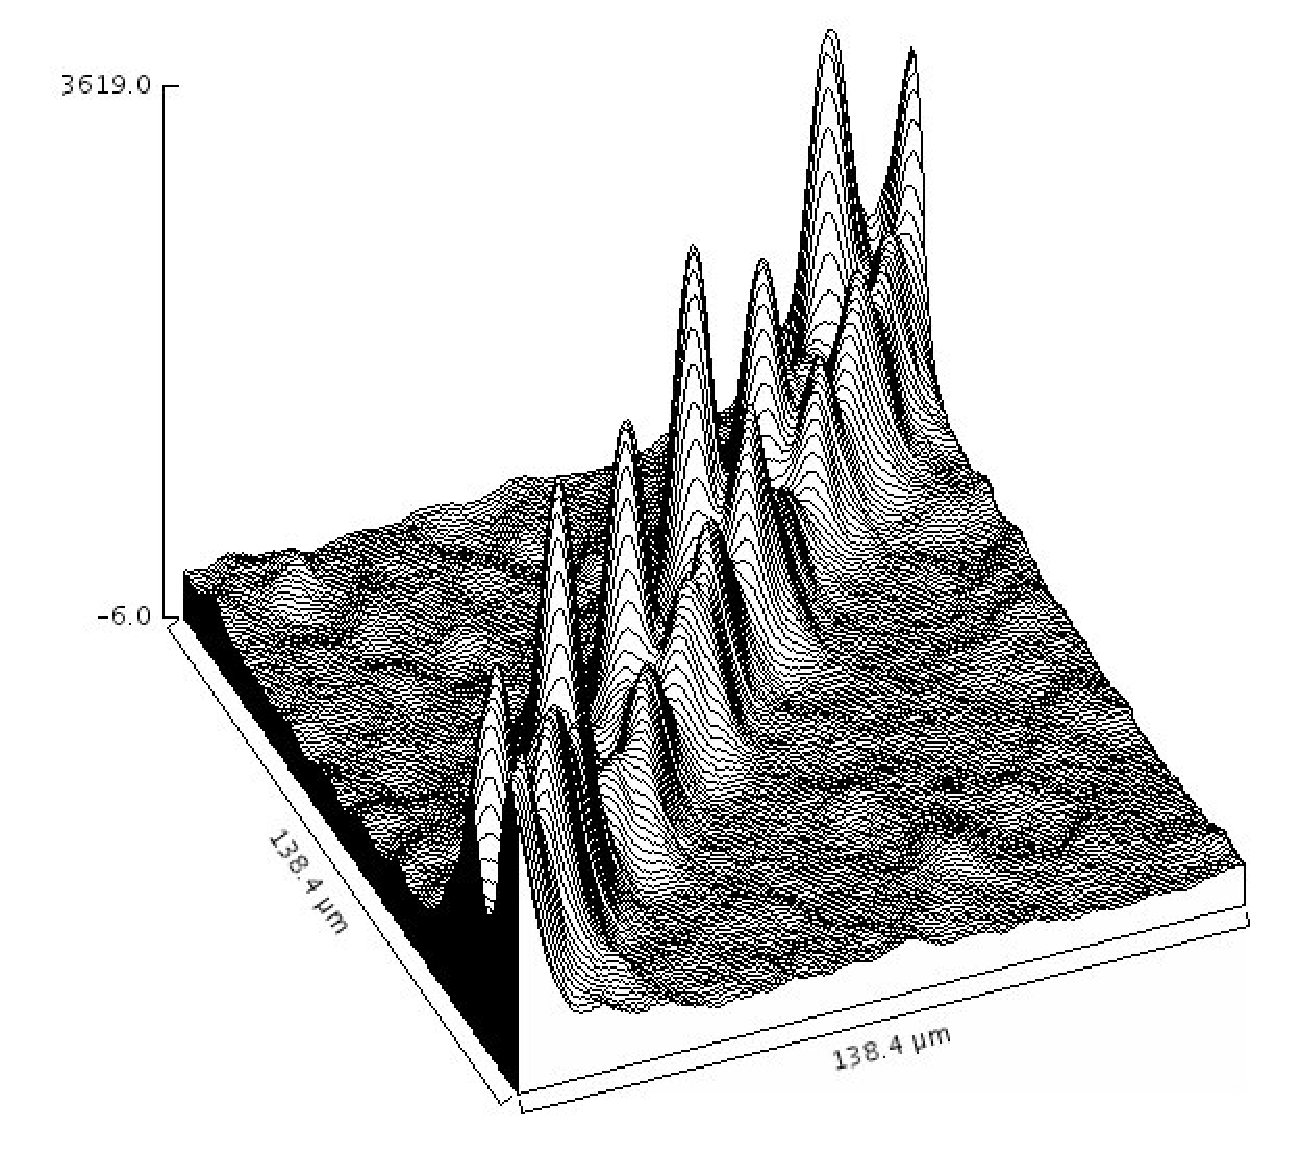
\includegraphics[width=7cm]{../app_dic/img/1219/auswert/1checker-height}
  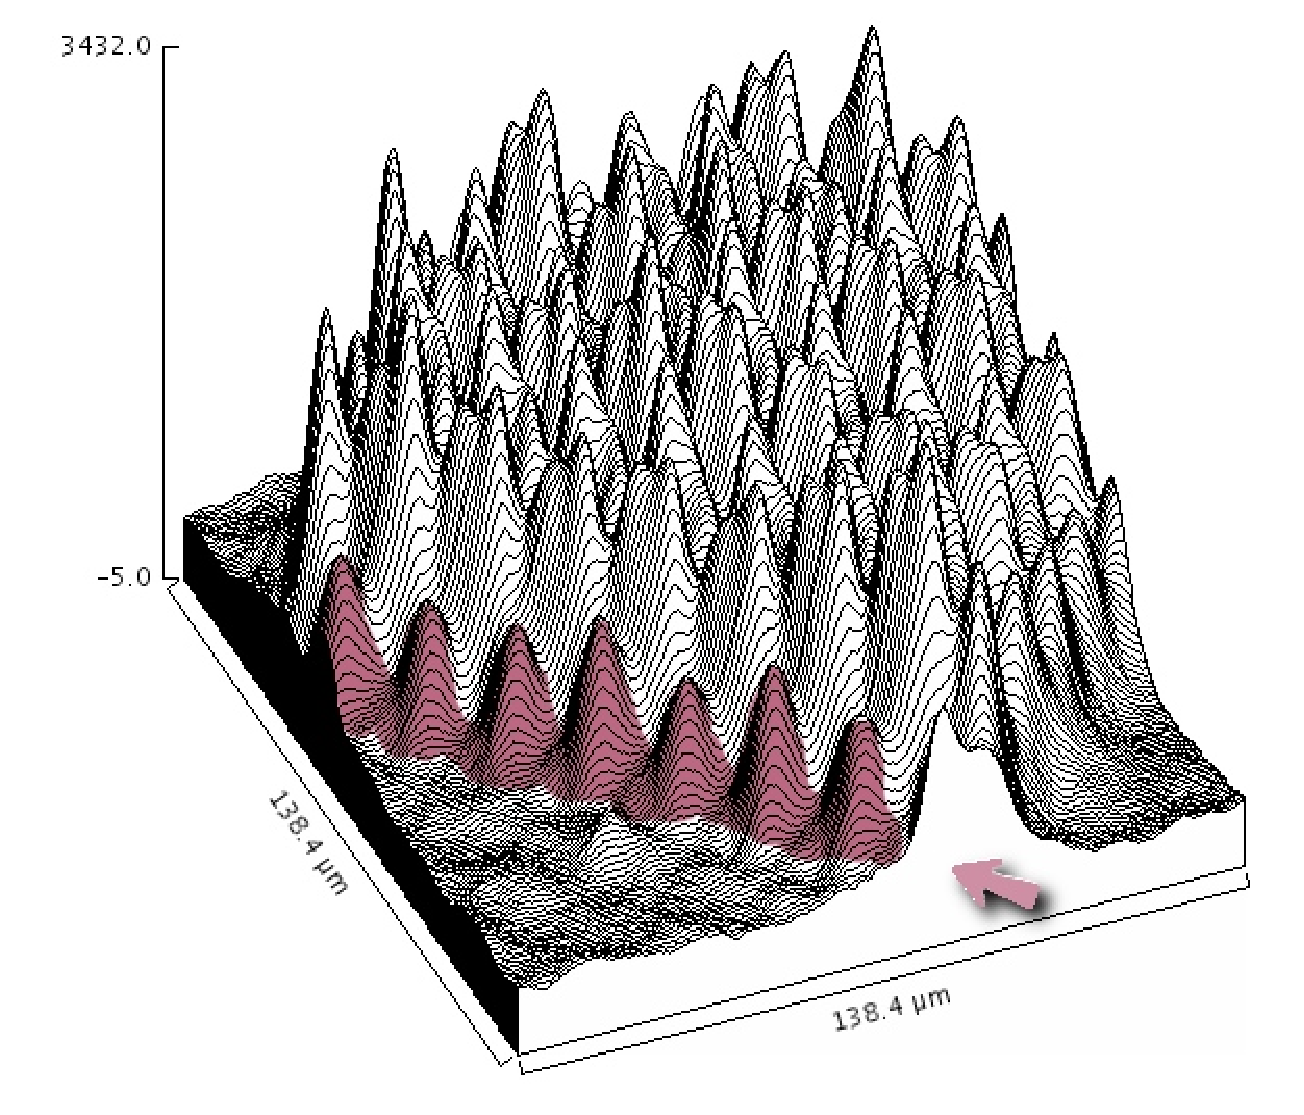
\includegraphics[width=7cm]{../app_dic/img/1219/auswert/2checker-height-arrow}
  \caption{ DIC image for a prism setting of $-45^\circ$ (a) and
    $+45^\circ$ (b). Below both images a cross section in the
    direction of the DIC shift is shown (along the line marked with
    1)). The horizontal lines in those graphs show the values
    $I_\textrm{max}$ and $I_\textrm{min}$ for contrast estimation. The
    contrast ratios are \unit[0.62]{} for (a) and \unit[0.65]{} for
    (b). The rectangular region that is marked with 2) in the images
    is shown in the bottom diagrams. These images were taken with two
    identical sequential DIC prisms (for $63\times/1.4$), a
    \unit[100]{mm} objective lens and a \unit[300]{mm} tube lens.}
  \label{fig:screen5}
\end{figure}

\figref{fig:screen5}~a) shows the corresponding image with
the prism turned by $90^\circ$ relative to the right image. The
displayed image on the MMA is the same black and white
checkerboard. According to the left diagram in \figref{fig:screen} one
would expect white lines perpendicular to the shift direction. The
image on the camera has these features and again one can make out the
dark lines in the centres of the pixels.

The contrast ratio for this experiment is only \unit[0.6] and also the
contrast in \figref{fig:screen5}~b) isn't much higher. This is
probably because two identical DIC prisms were used in sequence to
achieve twice the split (see \figref{fig:double-prism}). Without this
disputable trick a \unit[200]{mm} lens has to be used to get the
necessary $\unit[16]{\mu m}$ DIC split but then the Fourier pattern is
too big for the size of our DIC prisms. 
\begin{figure}[htb]
  \centering
  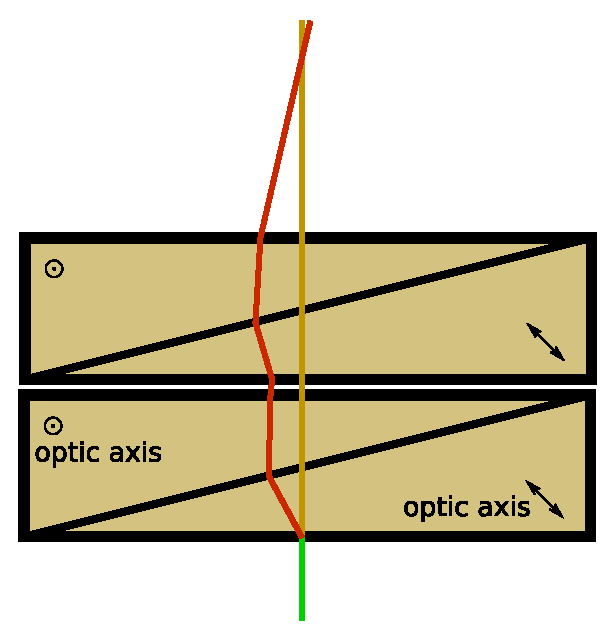
\includegraphics[width=5cm]{../app_dic/img/double-prism}
  \caption{Combination of two identical DIC prisms to increase the
    split. The prism in the experiments are for a $63\times/1.4$ oil
    immersion objective.}
  \label{fig:double-prism}
\end{figure}
\figref{fig:erika-overview} shows the gray value image that should be
displayed on the camera. The image that has to be displayed on the MMA
is shown in \figref{fig:erika-detail}~b) and
\figref{fig:erika-detail}~c) shows the result on the camera (for the
configuration with two DIC prisms).

In section section \ref{sec:size} some measurements for the setup with a
\unit[200]{mm} objective lens and only one prism are shown.
\begin{figure}[p]
  \centering
  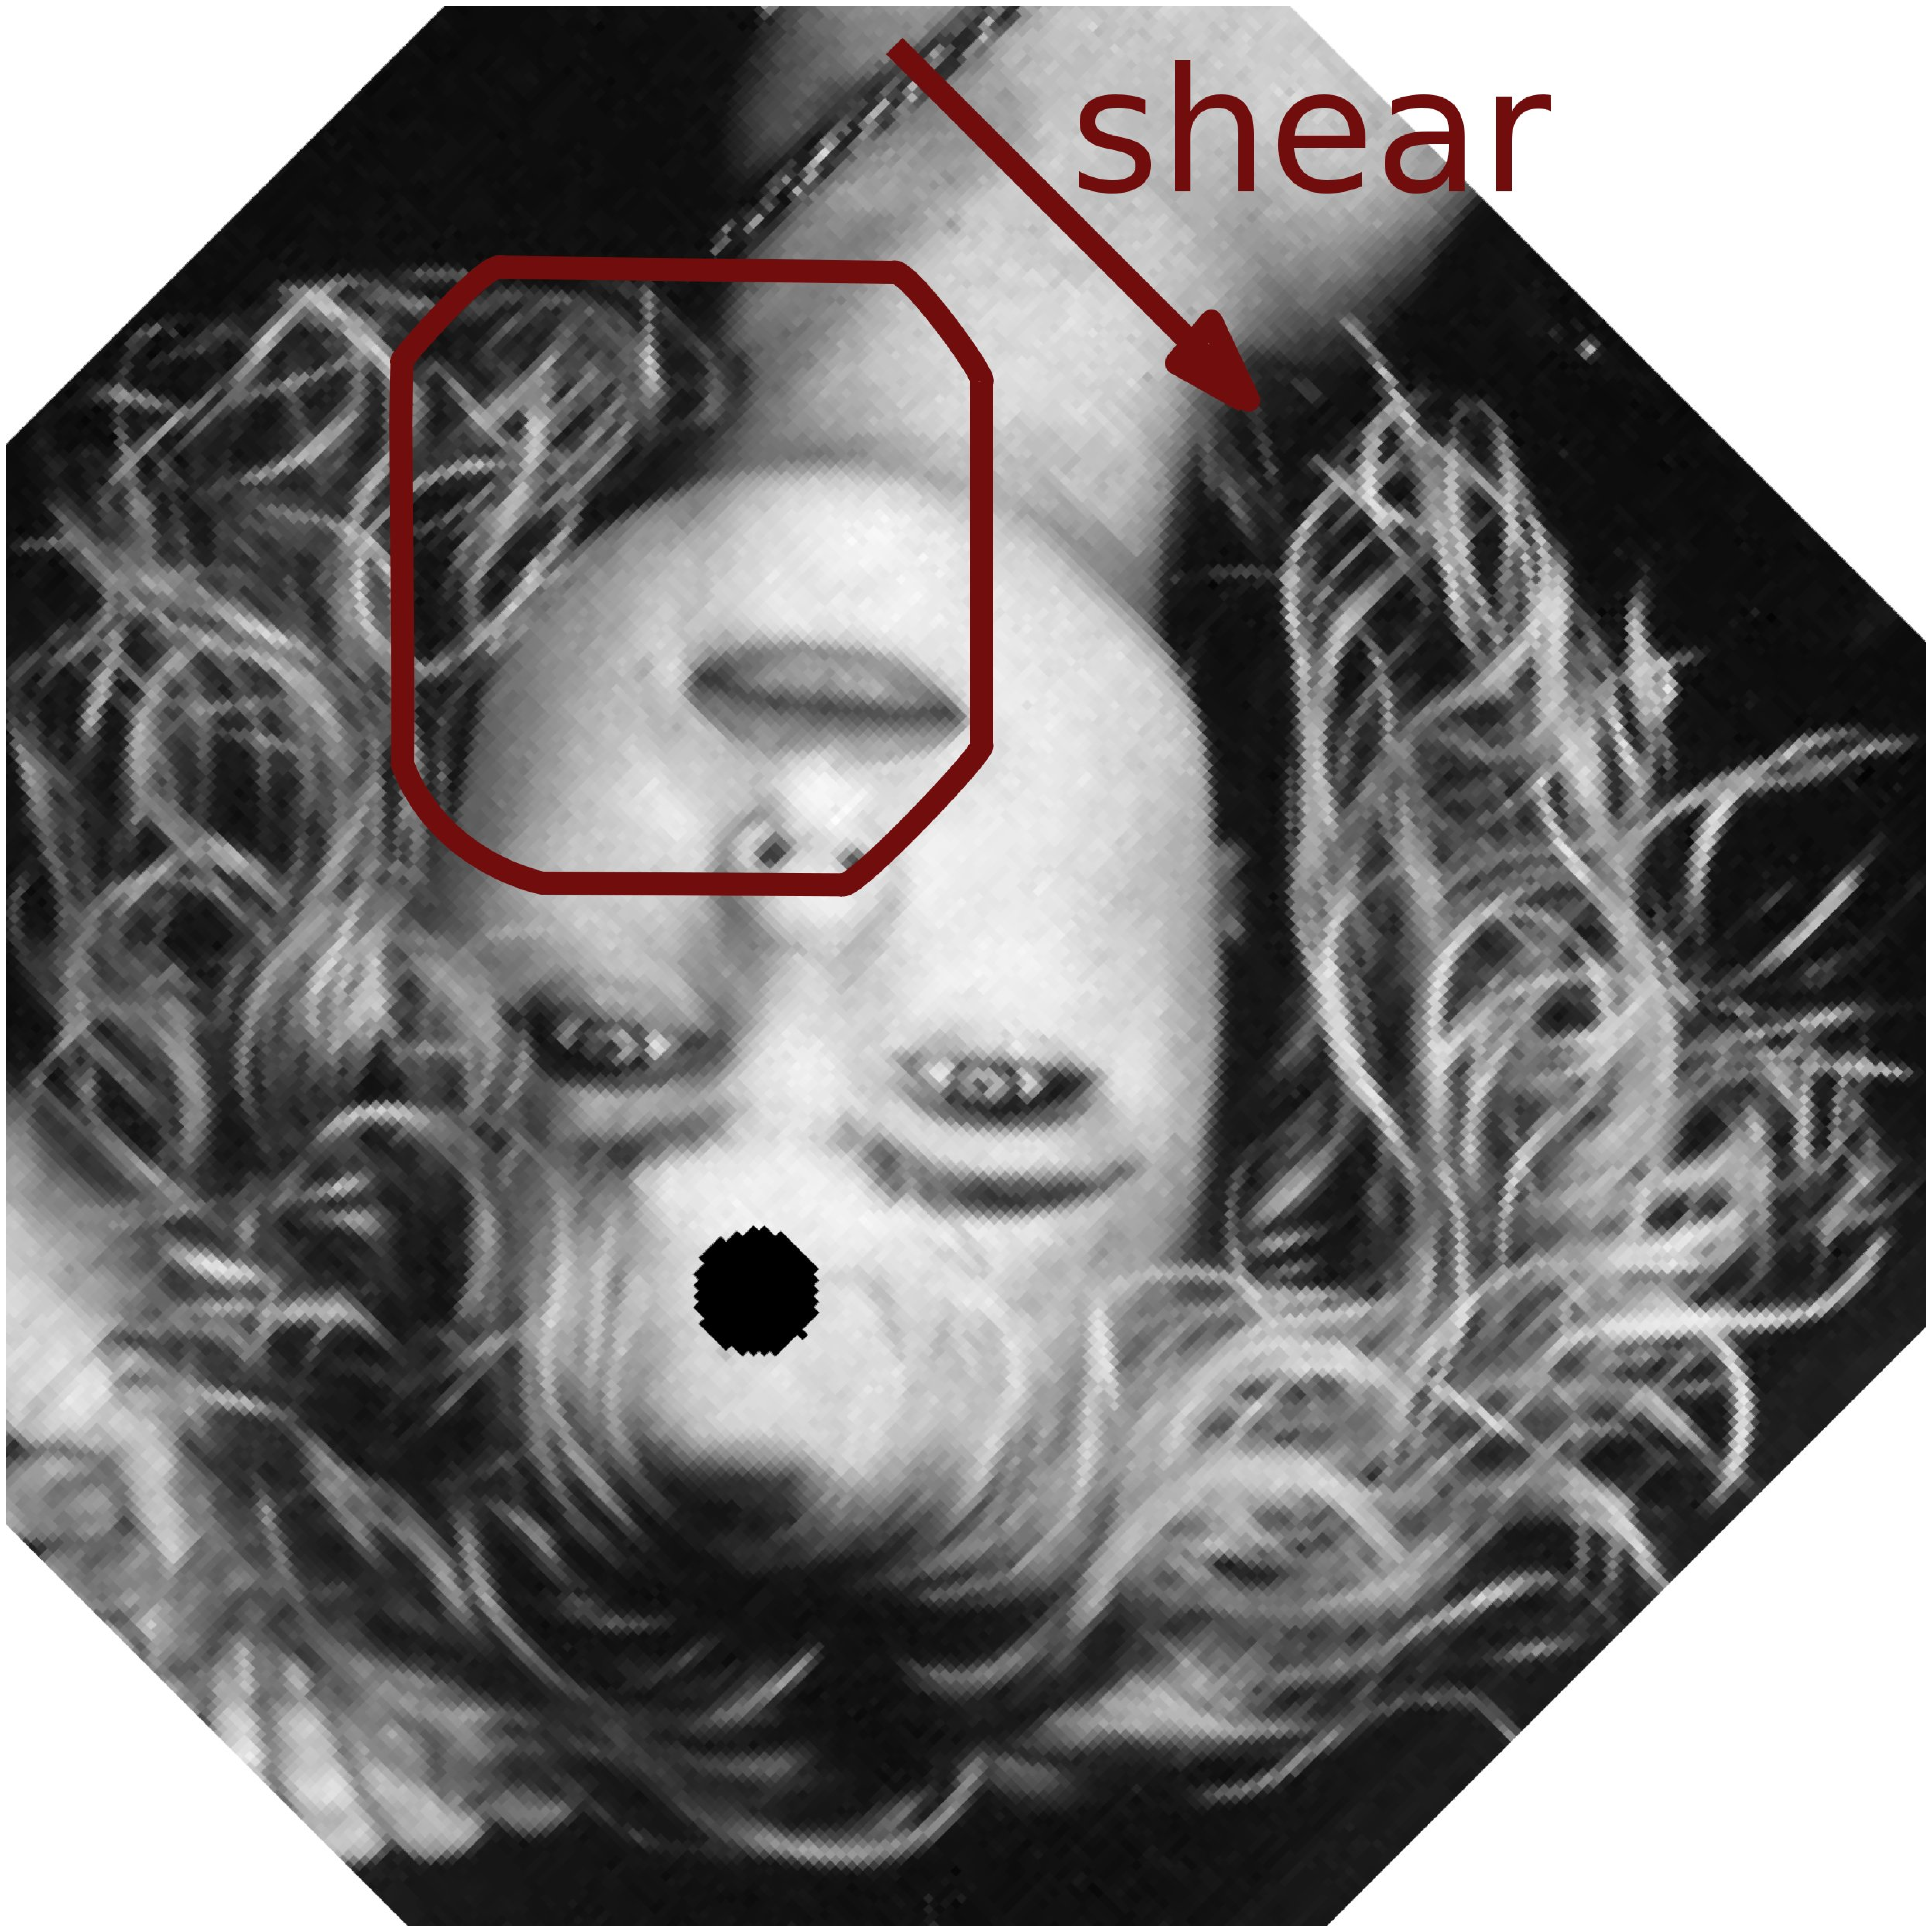
\includegraphics[width=4cm]{../app_dic/img/1219/auswert/erika-overview}
  \caption{The input image that should be displayed on the camera. The
    rectangular region is illuminated by the integrating rod and
    imaged on the CCD.}
  \label{fig:erika-overview}
\end{figure}

\begin{figure}[p]
  \centering
  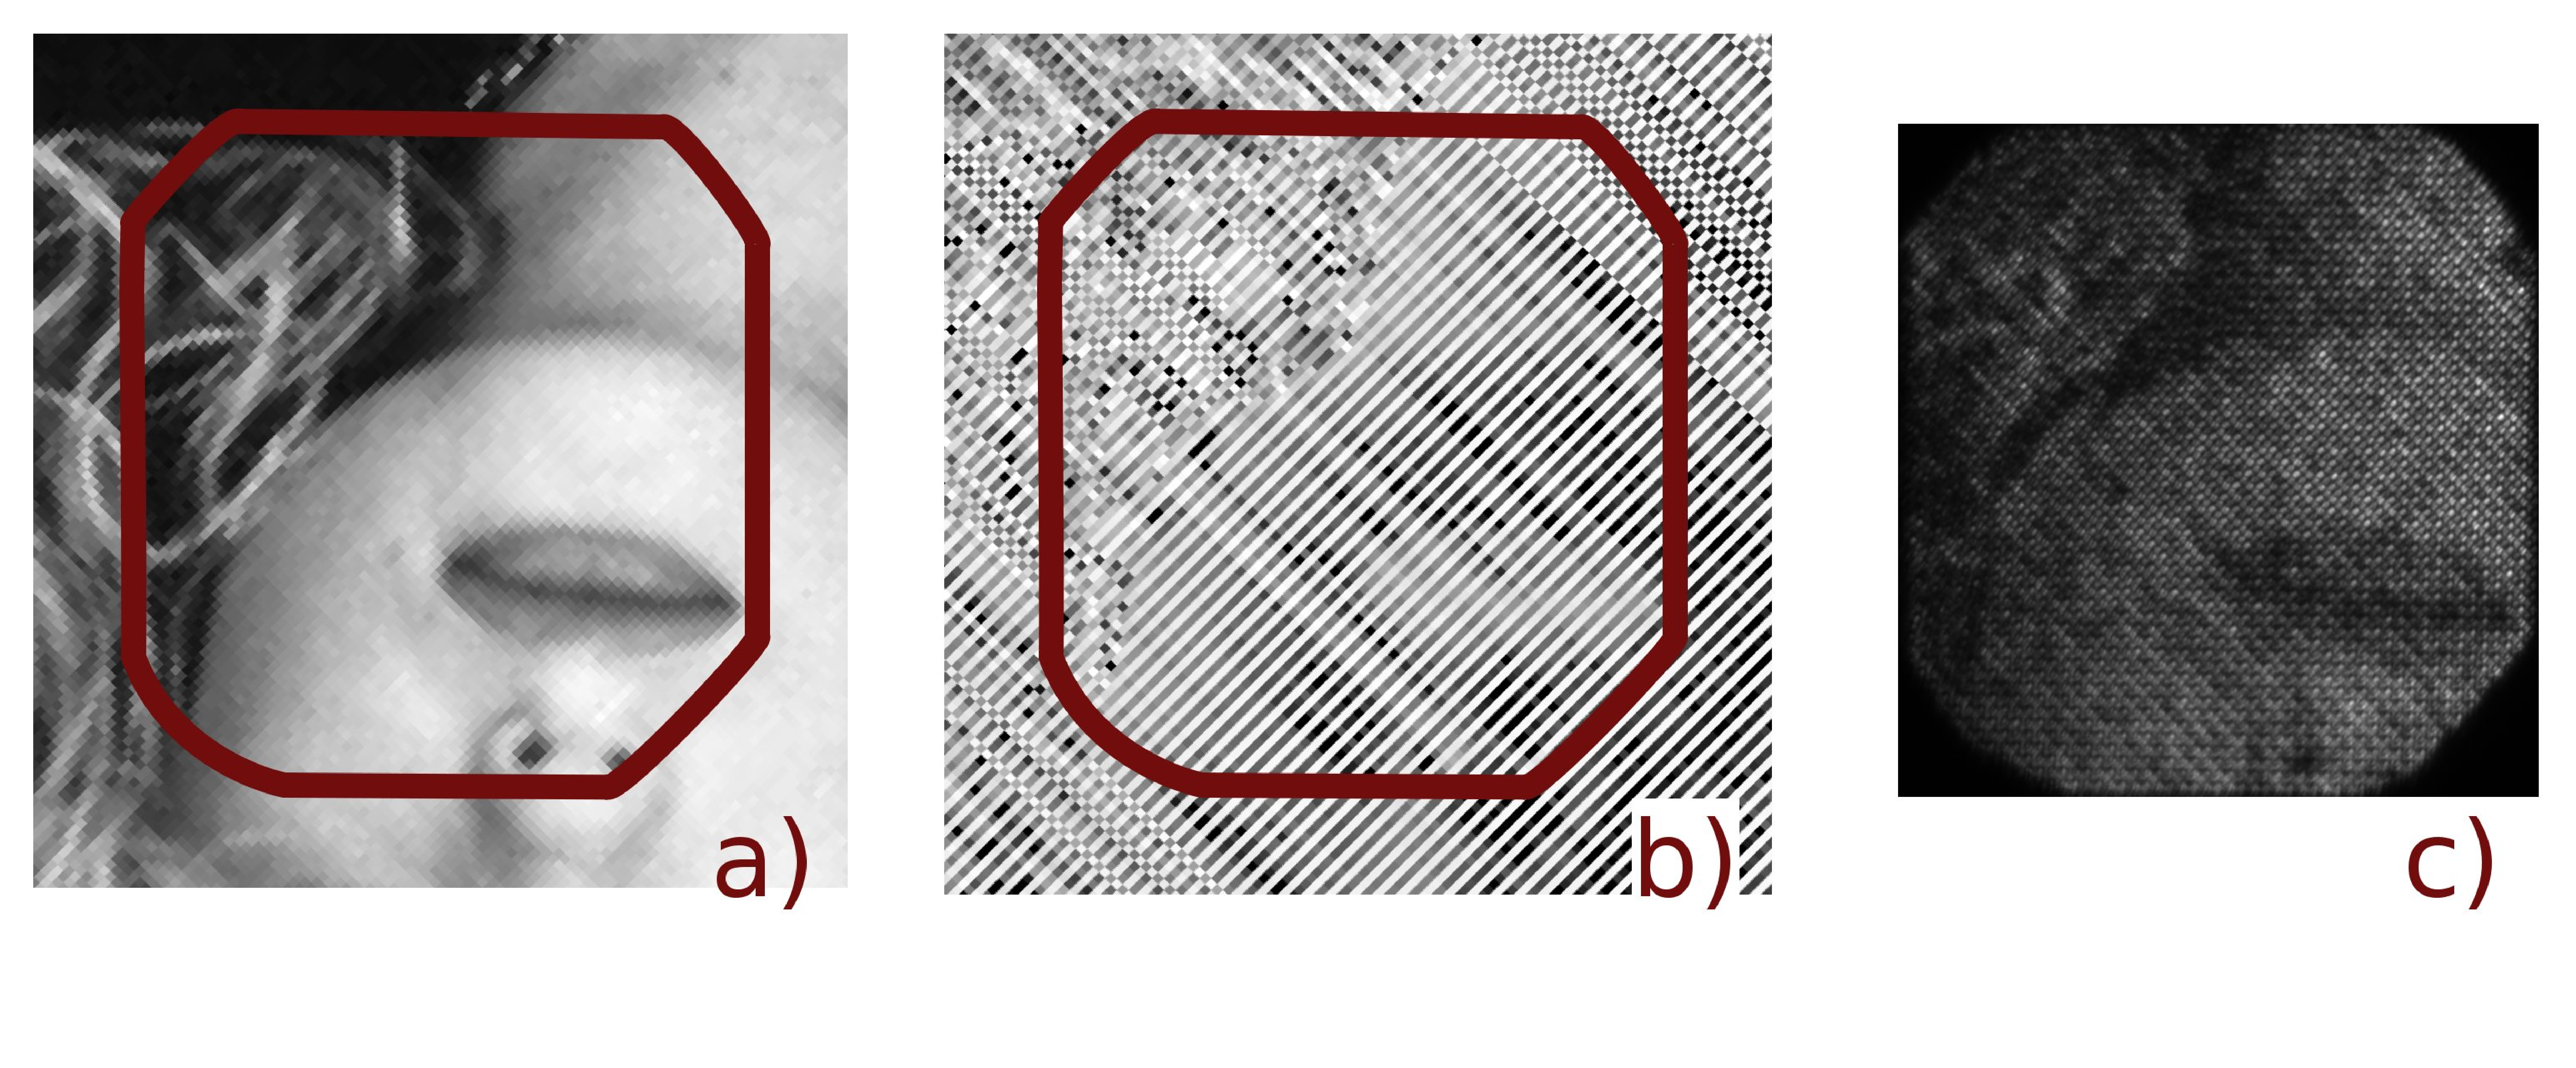
\includegraphics[width=.8\linewidth]{../app_dic/img/1219/auswert/erika-detail}
  \caption{{\bf (a)} Closeup of the input image. {\bf (b)} The
    precomputed (with the look up table algorithm) image that is
    displayed on the MMA. The DIC shift will occur from the left top
    towards the right bottom. Note that regions that are white in the
    input image have a grating structure with high contrast. {\bf (c)}
    The resulting image on the camera.}
  \label{fig:erika-detail}
\end{figure}
\newpage
\subsection{Effects of limited crystal size on DIC image}
\label{sec:size}
The split angle of the DIC prism defines the focal length of the
objective lens that needs to be used because the shift on the MMA must
be $\unit[16]{\mu m}$. Our prism with the biggest split needs a
\unit[200]{mm} lens. However the free aperture of the prism is only
\unit[10]{mm}. Therefore it is problematic to capture three orders in
the image on the camera. These orders are needed to form an
object-like image.

For \figref{fig:erikas} one DIC prism was used with a \unit[200]{mm}
objective lens. It is not possible to get the two outside orders with
their complete surrounding information through the prism. The relative
size of the diffraction pattern on the DIC prism aperture is shown on
top of the images in \figref{fig:erikas}. Note that the angular extend
of the illumination is indicated by the red spots in the Fourier
pattern.

The main advantage of the DIC method -- and here we didn't make use of
this -- is that the angular extend of the illumination can be
significantly increased. Then the red spots grow and may
overlap. However all of them should still pass through the DIC prism.

In this experiment most of the orders were cut off. This leads to some
artifacts that are more pronounced when the aperture of the prism is
artificially shrunken (with a circular aperture).

The experiment showed that the artifacts originate from line-like
image patterns that accidentally develop during our look-up table
algorithm. See \figref{fig:erika-streak-overview}) for a closeup of
one such region.  For this particular image it was possible to reduce
the number of line-like patterns on the face by starting the look up
table algorithm on a central column and then computing to the left and
the right.

However even with this trick there are still some phase jumps after
strong gray value discontinuities in the input image (see the red
arrows in \figref{fig:erika-streak-overview}). The only real solution
is to make the Nomarski prism bigger or use piston mirrors.

\begin{figure}[htb]
  \centering
  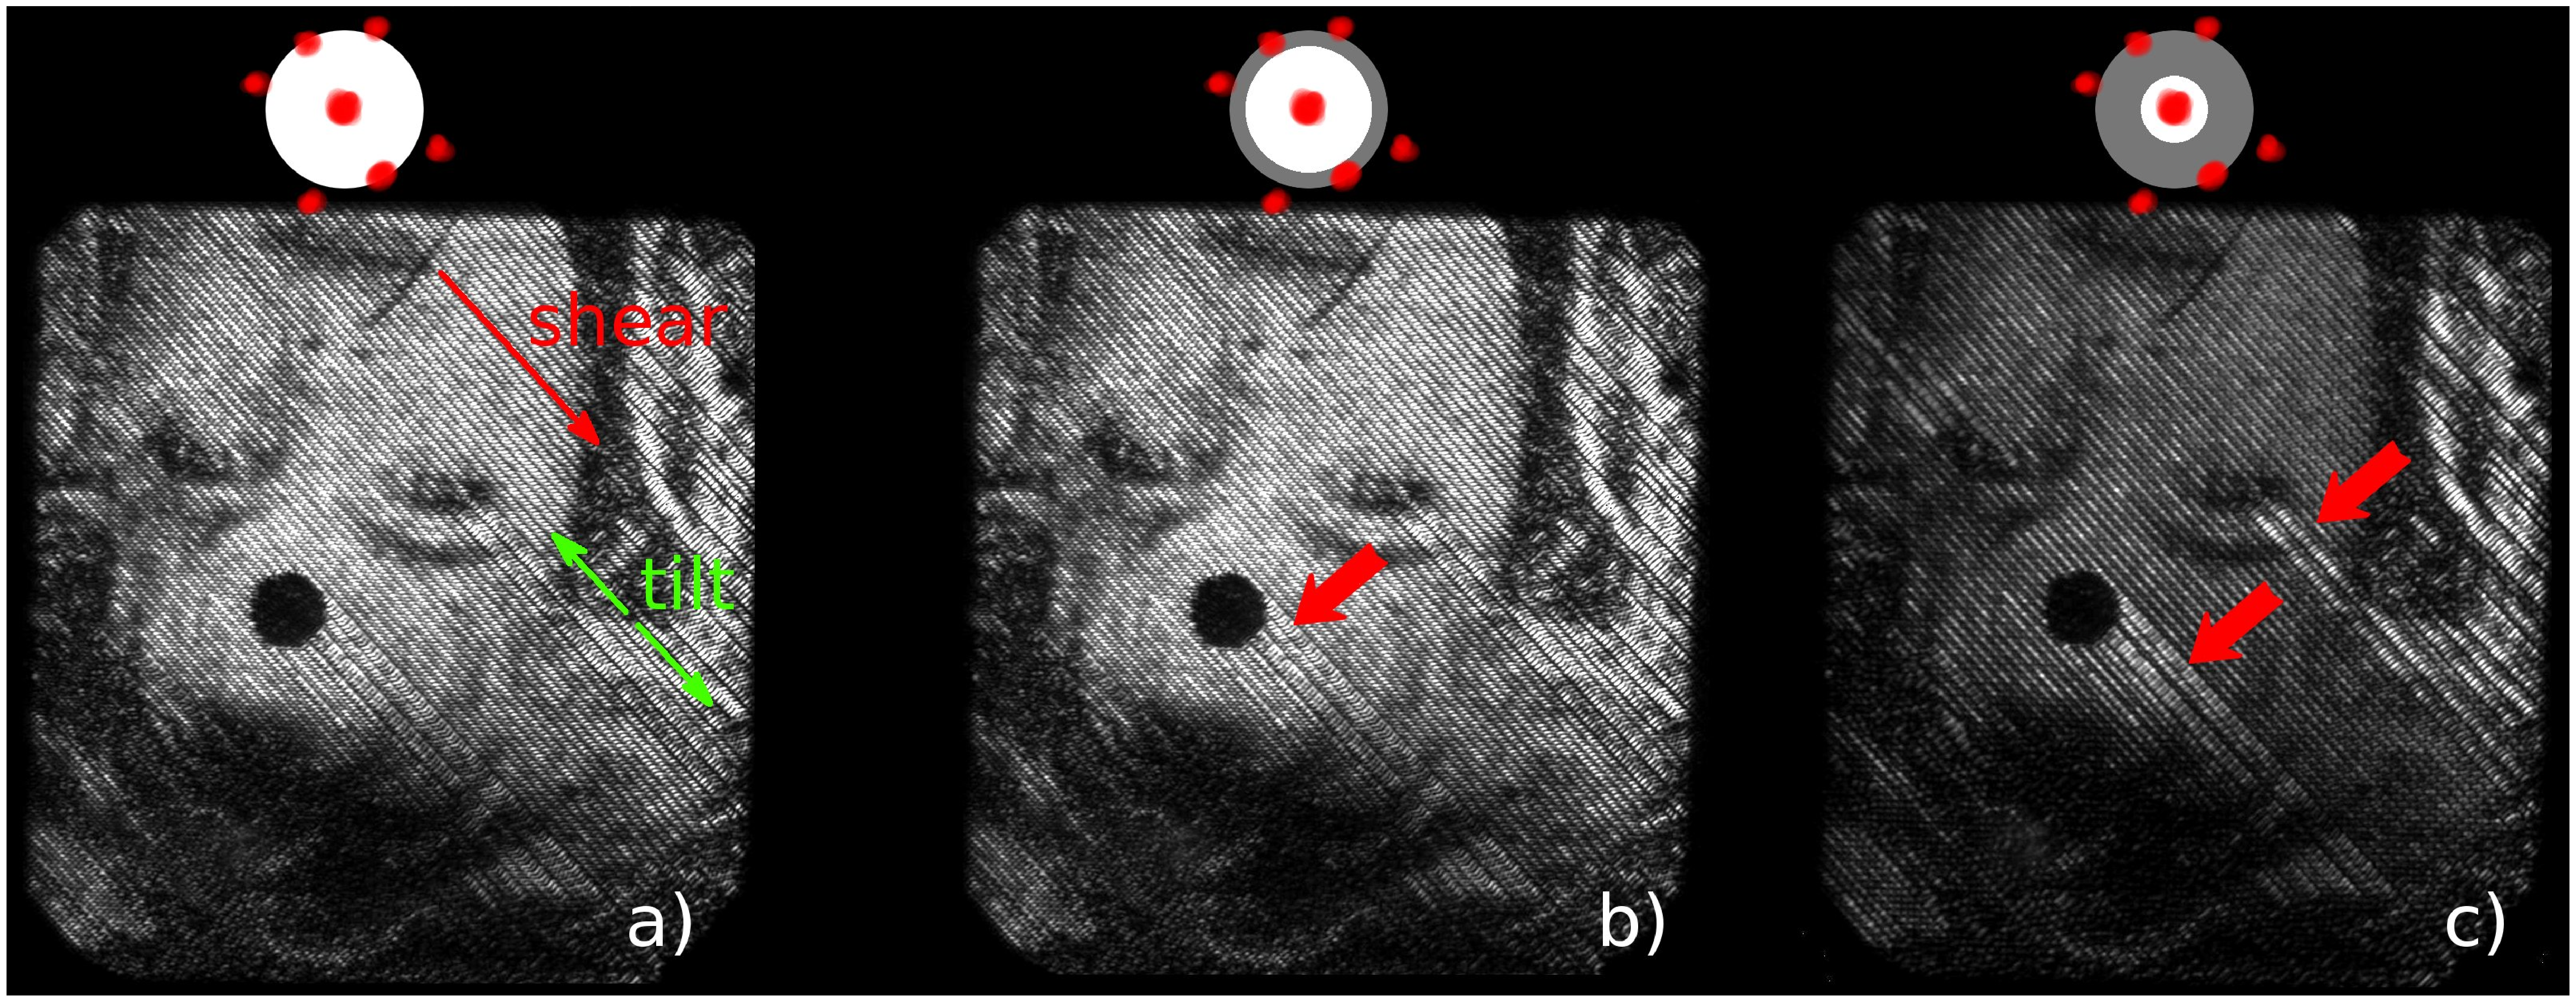
\includegraphics[width=.8\linewidth]{../app_dic/img/streaks2}
  \caption{These three images show artifacts in gray level images that
    arise when less than three orders contribute to the image. The
    diagram in the top shows the aperture diameter in relation to the
    Fourier pattern of the MMA device. Phase changes in the displayed
    MMA image (see \figref{fig:erika-streak-overview}) result in
    banding artifacts (see red arrows) for decreasing aperture
    diameter. These images were taken with one DIC prism (for
    $63\times\,,1.4$ micro objective) a \unit[200]{mm} objective lens
    and a \unit[500]{mm} tube lens.}
  \label{fig:erikas}
\end{figure}

\begin{figure}[p]
  \centering
  
\includegraphics[width=8cm]{../app_dic/img/1219/auswert/erika-streak-overview}
  \caption{This image is displayed on the MMA in order to create a
    gray value DIC image. The shear direction is from top left to
    bottom right. When neighbouring image values are black and white
    the resulting pixel on the camera will be bright. If the image
    values don't change (look e.g.\ at the inside of the black circle)
    the pixel will be dark on the camera. When a dark gray value is to
    be generated there are many gray value pairs that result in the
    same intensity after the DIC device. However, if not all Fourier
    orders contribute to the camera image this is not true. Especially
    phase steps (see red arrows) produce banding artifacts. Note that
    this image generates a gray value image without artifacts when the
    two DIC prisms with a \unit[100]{mm} lens are used.}
  \label{fig:erika-streak-overview}
\end{figure}

\section{Discussion}
The theoretical considerations lead to the conclusion that a piston
device possesses two significant advantages compared to the torsion
mirrors. The DIC prism has to be big enough so that at least three
orders of the diffraction pattern of the torsion mirrors can form an
image. Torsion mirrors always have a black line in the centre of the
pixel because here neighbouring mirrors have the same height. A piston
device therefore will achieve higher contrast at equivalent deflection
height and will need a smaller prism diameter.

For optimal performance it is crucial to have the MMA exactly in
focus. Currently it is very hard to focus the MMA as it is fixed to a
large printed circuit board with a heavy cable. After each focus
change the angle of the board generally has to be readjusted so that
the zero order returns back through the Nomarski prism. With the
generation-2 MMA this problem has been solved as the device is
connected to the circuit board by a flexible cable.

As an interesting application of the DIC method (other than improving
the contrast) it might be possible to determine characteristic
deflection curves for all mirrors of a device individually. One
approach would be to set all the mirrors parallel to the device
surface with a $+45^\circ$ DIC setting and then check for blackness
with a $-45^\circ$ setting and different voltages applied to
neighbouring mirrors. With a device that is calibrated in such a way
even better contrast will be possible, as mirror tilts can be adjusted
to be exactly equal (with an uncalibrated device there is some spread
due to manufacturing differences). At the time of the experiments no
programmable update of images was possible. Therefore no such iterative
calibration algorithm has been implemented.
